\documentclass[aspectratio=169,xcolor=table]{beamer}
\usepackage{hyperref}
\usepackage{tikz}
\usepackage{graphicx}
\usepackage{graphbox}
\usepackage{siunitx}
\usepackage[maxcitenames=6, url=false,doi=false]{biblatex}
\usepackage{subcaption}
\usepackage[outputdir=_build,draft=false]{minted}
\usepackage{pdfpc}

\usepackage{lmodern}
\usepackage{libertine}
\renewcommand\ttdefault{lmtt}

\usepackage{dirtree}
% Unsaturated
% \definecolor{cnt}{HTML}{C7C1C2}
% \definecolor{dir}{HTML}{DBDCE8}
% \definecolor{rev}{HTML}{E7F2F2}
% \definecolor{rel}{HTML}{FFFCCD}
% \definecolor{snp}{HTML}{F5F5F5}
% \definecolor{ori}{HTML}{FFFFFF}

% Saturated, darkened
% \definecolor{cnt}{HTML}{BBA3A7}
% \definecolor{dir}{HTML}{B7BAD9}
% \definecolor{rev}{HTML}{C3E3E3}
% \definecolor{rel}{HTML}{FFF89A}
% \definecolor{snp}{HTML}{E3E3E3}
% \definecolor{ori}{HTML}{FFFFFF}

% Saturated, darkened, improved
\definecolor{cnt}{HTML}{BFA6AA}
\definecolor{dir}{HTML}{CFD2F2}
\definecolor{rev}{HTML}{C3E3E3}
\definecolor{rel}{HTML}{FFF9A3}
\definecolor{snp}{HTML}{E3E3E3}
\definecolor{ori}{HTML}{FFFFFF}

\makeatletter
\pgfkeys{/tikz/.cd,
  tab height/.initial=3pt,
  tab width/.initial=10pt,
  tab slope/.initial=1.5pt,
  cover xoff/.initial=5pt,
  cover yoff/.initial=2pt,
}
%% Note: use '\setlength{\pgf@xd}{\pgf@xb}' rather than '\pgf@xd=\pgf@xb'
%% ??? for some reason \pgf@ytt etc. didn't work, but \pgf@ytt does
\newlength\pgf@ytt
\newlength\pgf@xe
\newlength\pgf@xf
\newlength\pgf@xg
\newlength\pgf@yg
\newlength\pgf@xh
%% this didn't work
\newlength\pgf@xo  %% note: \pgf@xx is pre-defined by pgf to mean something

%% from 95.2 Communicating with the Basic Layer via Macros
% \newdimen\pgf@xta \newdimen\pgf@xtb \newdimen\pgf@ytt
% \newdimen\pgf@xoa \newdimen\pgf@xob \newdimen\pgf@yoo
\pgfdeclareshape{document}{ % or 'directory'
  %% this is nearly a rectangle
  \inheritsavedanchors[from=rectangle]
  \inheritanchorborder[from=rectangle]
  \inheritanchor[from=rectangle]{center}
  \inheritanchor[from=rectangle]{north}
  \inheritanchor[from=rectangle]{south}

  \savedmacro\tabheight{%
    \edef\tabheight{\pgfkeysvalueof{/tikz/tab height}}%
  }
  \savedmacro\tabwidth{%
    \edef\tabwidth{\pgfkeysvalueof{/tikz/tab width}}%
  }
  \savedmacro\tabslope{%
    \edef\tabslope{\pgfkeysvalueof{/tikz/tab slope}}%
  }
  \savedmacro\coverxoff{%
    \edef\coverxoff{\pgfkeysvalueof{/tikz/cover xoff}}%
  }
  \savedmacro\coveryoff{%
    \edef\coveryoff{\pgfkeysvalueof{/tikz/cover yoff}}%
  }
  %% this didn't work; probably needs \pgf@process somewhere...
  % \setlength{\pgf@xo}{\coverxoff}
  % \setlength{\pgf@xo}{0.5\pgf@xo}

  %% this didn't work either
  % \setlength{\pgf@xo}{2pt}
  % \advance\pgf@xo by \coverxoff\relax

  %% this didn't work either
  % \pgf@xx=0pt
  % \advance\pgf@xx by \coverxoff\relax
  % \pgf@xx=0.5\pgf@xx

  %% fallback, so this at least compile
  %% but moves text, because \pgf@xx is sed for node contents positioning
  % \pgf@xx=2pt % this should be 0.5 of \coverxoff

  % \inheritanchor[from=rectangle]{west}
  \anchor{west}{
    \pgf@process{\northeast}%
    \pgf@ya=.5\pgf@y%
    \pgf@process{\southwest}%
    \pgf@y=.5\pgf@y%
    % \advance\pgf@y by  \pgf@ya%
    % \advance\pgf@x by -2pt%
  }
  % \inheritanchor[from=rectangle]{east}
  \anchor{east}{%
    \pgf@process{\southwest}%
    \pgf@ya=.5\pgf@y%
    \pgf@process{\northeast}%
    \pgf@y=.5\pgf@y%
    % \advance\pgf@y by  \pgf@ya%
    % \advance\pgf@x by  2pt%
  }
  \backgroundpath{% this is new
    %% store lower left in xa/ya and upper right in xb/yb
    \southwest \pgf@xa=\pgf@x \pgf@ya=\pgf@y
    \northeast \pgf@xb=\pgf@x \pgf@yb=\pgf@y
    %% correction due to open front cover
    % \advance\pgf@xa by -2pt
    % \advance\pgf@xb by -2pt
    %%
    %% compute edges of the "divider tab" in the back cover
    %%
    \setlength{\pgf@ytt}{\pgf@yb}
    \advance\pgf@ytt by \tabheight
    \setlength{\pgf@xe}{\pgf@xa}
    \advance\pgf@xe by \tabwidth % or make it dependent on box width
    \setlength{\pgf@xf}{\pgf@xe}
    \advance\pgf@xf by \tabslope % or make it dependent on divider height
    %%
    %% compute edges of second cover of a folder ("open" cover)
    %%
    \setlength{\pgf@xg}{\pgf@xa}
    \advance\pgf@xg by \coverxoff % perhaps as an angle of open
    \setlength{\pgf@xh}{\pgf@xb}
    \advance\pgf@xh by \coverxoff
    \setlength{\pgf@yg}{\pgf@yb}
    \advance\pgf@yg by-\coveryoff % perhaps as an angle of open
    %%
    %% construct main path
    \pgfpathmoveto{\pgfpoint{\pgf@xa}{\pgf@ya}}
    \pgfpathlineto{\pgfpoint{\pgf@xa}{\pgf@ytt}}
    \pgfpathlineto{\pgfpoint{\pgf@xe}{\pgf@ytt}}
    \pgfpathlineto{\pgfpoint{\pgf@xf}{\pgf@yb}}
    \pgfpathlineto{\pgfpoint{\pgf@xb}{\pgf@yb}}
    \pgfpathlineto{\pgfpoint{\pgf@xb}{\pgf@ya}} % break for open cover
    \pgfpathmoveto{\pgfpoint{\pgf@xb}{\pgf@ya}}
    % \pfgpathlineto{\pgfpoint{\pgf@xa}{\pgf@ya}} % ??? causes error ???
    \pgfpathclose
    %% construct secondary path
    \pgfpathmoveto{\pgfpoint{\pgf@xa}{\pgf@ya}}
    % \pgfpathlineto{\pgfpoint{\pgf@xg}{\pgf@yg}}
    % \pgfpathlineto{\pgfpoint{\pgf@xh}{\pgf@yg}}
    \pgfpathlineto{\pgfpoint{\pgf@xb}{\pgf@ya}}
    \pgfpathclose
  }
}
\makeatother

\usetikzlibrary{calc}
\usepackage{etoolbox}

\pgfdeclarelayer{background}
\pgfdeclarelayer{foreground}
\pgfdeclarelayer{sankeydebug}
\pgfsetlayers{background,main,foreground,sankeydebug}

\newif\ifsankeydebug

\newenvironment{sankeydiagram}[1][]{

  \def\sankeyflow##1##2{% sn, en
    \path[sankey fill]
    let
    \p1=(##1.north east),\p2=(##1.south east),
    \n1={atan2(\y1-\y2, \x1-\x2)-90},
    \p3=(##2.north west),\p4=(##2.south west),
    \n2={atan2(\y3-\y4, \x3-\x4)+90}
    in
    (\p1) to[out=\n1,in=\n2] (\p3) --
    (\p4) to[in=\n1,out=\n2] (\p2) -- cycle;
    \draw[sankey draw]
    let
    \p1=(##1.north east),\p2=(##1.south east),
    \n1={atan2(\y1-\y2, \x1-\x2)-90},
    \p3=(##2.north west),\p4=(##2.south west),
    \n2={atan2(\y3-\y4, \x3-\x4)+90}
    in
    (\p1) to[out=\n1,in=\n2] (\p3)
    (\p4) to[in=\n1,out=\n2] (\p2);
  }


  \tikzset{
    sankey tot length/.store in=\sankeytotallen,
    sankey tot quantity/.store in=\sankeytotalqty,
    sankey min radius/.store in=\sankeyminradius,
    sankey arrow length/.store in=\sankeyarrowlen,
    sankey debug/.is if=sankeydebug,
    sankey debug=false,
    sankey flow/.style={
      to path={
        \pgfextra{
          \pgfinterruptpath
          \edef\sankeystart{\tikztostart}
          \edef\sankeytarget{\tikztotarget}
          \sankeyflow{\sankeystart}{\sankeytarget}
          \endpgfinterruptpath
        }
      },
    },
    sankey node/.style={
      inner sep=0,minimum height={sankeyqtytolen(##1)},
      minimum width=0,draw=none,line width=0pt,
    },
    % sankey angle
    sankey angle/.store in=\sankeyangle,
    % sankey default styles
    sankey fill/.style={line width=0pt,fill,white},
    sankey draw/.style={draw=black,line width=.4pt},
  }

  \newcommand\sankeynode[4]{%prop,orientation,name,pos
    \node[sankey node=##1,rotate=##2] (##3) at (##4) {};
    \ifsankeydebug
    \begin{pgfonlayer}{sankeydebug}
      \draw[red,|-|] (##3.north west) -- (##3.south west);
      \pgfmathsetmacro{\len}{sankeyqtytolen(##1)/3}
      \draw[red] (##3.west)
      -- ($(##3.west)!\len pt!90:(##3.south west)$)
      node[font=\tiny,text=black] {##3};
    \end{pgfonlayer}
    \fi
  }

  \newcommand\sankeynodestart[4]{%prop,orientation,name,pos
    \sankeynode{##1}{##2}{##3}{##4}
    \begin{scope}[shift={(##3)},rotate=##2]
      \path[sankey fill]
      (##3.north west) -- ++(-\sankeyarrowlen,0)
      -- ([xshift=-\sankeyarrowlen/6]##3.west)
      -- ([xshift=-\sankeyarrowlen]##3.south west)
      -- (##3.south west) -- cycle;
      \path[sankey draw]
      (##3.north west) -- ++(-\sankeyarrowlen,0)
      -- ([xshift=-\sankeyarrowlen/6]##3.west)
      -- ([xshift=-\sankeyarrowlen]##3.south west)
      -- (##3.south west);
    \end{scope}
  }

  \newcommand\sankeynodeend[4]{%prop,orientation,name,pos
    \sankeynode{##1}{##2}{##3}{##4}
    \begin{scope}[shift={(##3)},rotate=##2]
      \path[sankey fill]
      (##3.north east)
      -- ([xshift=\sankeyarrowlen]##3.east)
      -- (##3.south west) -- cycle;
      \path[sankey draw]
      (##3.north east)
      -- ([xshift=\sankeyarrowlen]##3.east)
      -- (##3.south west);
    \end{scope}
  }

  \newcommand\sankeyadvance[3][]{%newname,name,distance
    \edef\name{##2}
    \ifstrempty{##1}{
      \def\newname{##2}
      \edef\name{##2-old}
      \path [late options={name=##2,alias=\name}];
    }{
      \def\newname{##1}
    }
    \path
    let
    % sankey node angle
    \p1=(##2.north east),
    \p2=(##2.south east),
    \n1={atan2(\y1-\y2, \x1-\x2)-90},
    % sankey prop
    \p3=($(\p1)-(\p2)$),
    \n2={sankeylentoqty(veclen(\x3,\y3))},
    % next position
    \p4=($(##2.east)!##3!-90:(##2.north east)$)
    in
    \pgfextra{
      \pgfmathsetmacro{\prop}{\n2}
      \pgfinterruptpath
      \sankeynode{\prop}{\n1}{\newname}{\p4}
      \path (\name) to[sankey flow] (\newname);
      \endpgfinterruptpath
    };
  }

  \newcommand\sankeyturn[3][]{%newname,name,angle
    \edef\name{##2}
    \ifstrempty{##1}{
      \def\newname{##2}
      \edef\name{##2-old}
      \path [late options={name=##2,alias=\name}];
    }{
      \def\newname{##1}
    }
    \ifnumgreater{##3}{0}{
      \path
      let
      % sankey node angle
      \p1=(##2.north east),
      \p2=(##2.south east),
      \p3=($(\p1)!-\sankeyminradius!(\p2)$),
      \n1={atan2(\y1-\y2, \x1-\x2)-90},
      % sankey prop
      \p4=($(\p1)-(\p2)$),
      \n2={sankeylentoqty(veclen(\x4,\y4))},
      \p5=(##2.east),
      \p6=($(\p3)!1!##3:(\p5)$)
      in
      \pgfextra{
        \pgfmathsetmacro{\prop}{\n2}
        \pgfinterruptpath
        % \fill[red] (\p3) circle (2pt);
        % \fill[blue](\p6) circle (2pt);
        \sankeynode{\prop}{\n1+##3}{\newname}{\p6}
        \path (\name) to[sankey flow] (\newname);
        \endpgfinterruptpath
      };
    }{
      \path
      let
      % sankey node angle
      \p1=(##2.south east),
      \p2=(##2.north east),
      \p3=($(\p1)!-\sankeyminradius!(\p2)$),
      \n1={atan2(\y1-\y2, \x1-\x2)+90},
      % sankey prop
      \p4=($(\p1)-(\p2)$),
      \n2={sankeylentoqty(veclen(\x4,\y4))},
      \p5=(##2.east),
      \p6=($(\p3)!1!##3:(\p5)$)
      in
      \pgfextra{
        \pgfmathsetmacro{\prop}{\n2}
        \pgfinterruptpath
        % \fill[red] (\p3) circle (2pt);
        % \fill[blue](\p6) circle (2pt);
        \sankeynode{\prop}{\n1+##3}{\newname}{\p6}
        \path (\name) to[sankey flow] (\newname);
        \endpgfinterruptpath
      };
    }
  }

  \newcommand\sankeyfork[2]{%name,list of forks
    \def\name{##1}
    \def\listofforks{##2}
    \xdef\sankeytot{0}
    \path 
    let
    % sankey node angle
    \p1=(\name.north east),
    \p2=(\name.south east),
    \n1={atan2(\y1-\y2, \x1-\x2)-90},
    % sankey prop
    \p4=($(\p1)-(\p2)$),
    \n2={sankeylentoqty(veclen(\x4,\y4))}
    in
    \pgfextra{
      \pgfmathsetmacro{\iprop}{\n2}
    }
    \foreach \prop/\name[count=\c] in \listofforks {
      let
      \p{start \name}=($(\p1)!\sankeytot/\iprop!(\p2)$),
      \n{nexttot}={\sankeytot+\prop},
      \p{end \name}=($(\p1)!\n{nexttot}/\iprop!(\p2)$),
      \p{mid \name}=($(\p{start \name})!.5!(\p{end \name})$)
      in
      \pgfextra{
        \xdef\sankeytot{\n{nexttot}}
        \pgfinterruptpath
        \sankeynode{\prop}{\n1}{\name}{\p{mid \name}}
        \endpgfinterruptpath
      }
    }
    \pgfextra{
      \pgfmathsetmacro{\diff}{abs(\iprop-\sankeytot)}
      \pgfmathtruncatemacro{\finish}{\diff<0.01?1:0}
      \ifnumequal{\finish}{1}{}{
        \message{*** Warning: bad sankey fork (maybe)...}
        \message{\iprop-\sankeytot}
      }
    };
  }

  \tikzset{
    % default values,
    declare function={
      sankeyqtytolen(\qty)=\qty/\sankeytotalqty*\sankeytotallen;
      sankeylentoqty(\len)=\len/\sankeytotallen*\sankeytotalqty;
    },
    sankey tot length=100pt,
    sankey tot quantity=100,
    sankey min radius=30pt,%
    sankey arrow length=10pt,%
    % user values
    #1}
}{
}

\input{../tikz/swh.tikzstyles}
\input{../tikz/swh.tikzdefs}

\definecolor{palegrey}{RGB}{242, 242, 244}
\definecolor{SwhLightRed}{cmyk}{.0,.89,.84,.07}

\setbeamercolor{background canvas}{bg=palegrey}
\useinnertheme{rounded}
\useoutertheme{shadow}
% \useoutertheme{infolines}
\usecolortheme{orchid}
\usecolortheme{whale}
\usecolortheme[named=SwhLightRed]{structure}

\setbeamerfont{footline}{series=\bfseries}
\setbeamertemplate{page number in head/foot}[totalframenumber]
\setbeamertemplate{navigation symbols}{}
\setbeamertemplate{bibliography item}[article]

\rowcolors[]{1}{blue!10}{blue!05}

\titlegraphic{%
    \hfill%
    
\includegraphics[align=c, width=0.3\textwidth]{../img/frontmatter/uni_paris}%
    \hfill%
    
\includegraphics[align=c, width=0.20\textwidth]{../img/frontmatter/inria.pdf}%
    \hfill%
    
\includegraphics[align=c, width=0.3\textwidth]{../img/frontmatter/SWH-logo}
    \hfill%
}

\AtBeginSection[]{%
    \begin{frame}
        \frametitle{Table of Contents}
        \tableofcontents[currentsection]
    \end{frame}
}

\setbeamertemplate{headline}{}


\title[Organizing the graph of public software development]{Organizing the graph of public software development for large-scale mining}
\subtitle{PhD Thesis Defense}
\author{Antoine \textsc{Pietri}}
\institute{Inria, Paris}
\date{November 5, 2021}

\hypersetup{%
    pdfauthor={Antoine Pietri},
    pdftitle={Organizing the graph of public software development for
        large-scale mining},
    pdfkeywords={empirical software engineering, source code, open source
        software, version control system, digital preservation, graph topology,
        graph
    compression},
    pdflang={English}
}

\addbibresource{../thesis.bib}

\begin{document}
    \pdfpcnote{%
        Welcome to my defense, I'm going to present what I've been working
        on during my PhD, under the supervision of my advisor, Stefano
        Zacchiroli.  Before discussing my subject, I first need to give a
        bit of context.
    }
    \maketitle

    \section*{Context}
    % presentation
    % universal software mining

    \begin{frame}
        \frametitle{Software Mining}

        \pdfpcnote{%
            I worked in the field of empirical software engineering, and more
            specifically a field called "software mining". The goal
            is to study existing software repositories in a systematic way to
            try to extract knowledge and **uncover patterns** in software
            development and in the **social processes that govern it**, in the
            goal of improving these practices.
            \\\\
            This field has a lot of applications, like automated bug fixing,
            code completion or finding unmaintained dependencies. Because of
            this potential, it has drawn a lot of interest from computer
            science researchers.
        }

        \begin{block}{Definition}
            \textbf{Software mining}: studying existing software repositories
            to help improve software development processes and practices.
            % all the byproducts of software development
            % improve the software of tomorrow
            % inform development best practices
        \end{block}

        \begin{block}{Applications}
            \begin{itemize}
                \item Software health, software evolution
                \item Automated bug detection
                \item Automated vulnerability repair
                \item Code autocompletion
                \item Clone detection
                \item License compliance
                \item …
            \end{itemize}
        \end{block}
    \end{frame}

    \begin{frame}
        \frametitle{Universal Software Mining}

        \pdfpcnote{%
            Initially, software mining studies were done at a relatively
            small scale, only individual projects or a dozen related projects.
            Then it started growing in scale, with researchers analyzing
            thousands of repositories at once or even sometimes up to entire
            ecosystems. This allowed us to have a more and more exhaustive
            understanding of software development processes.
            \\\\
            The main question that initiated the work I'm presenting here is:
            could we go even further? Could we provide a way to run empirical
            studies on all the body of public software development?
            \\\\
            This would be really impactful for the software mining field. It
            would **reduce the barriers of entry** for researchers, who
            wouldn't have to do all the manual data crawling themselves. It
            would make it really easy to replicate studies, and give us a more
            complete/exhaustive view on development practices and social
            processes.
        }

        \begin{block}{Current scale of software mining studies}
            \begin{itemize}
                \item Individual projects
                \item Up to thousands of popular repositories (e.g., ``top
                    1000 by stars'')
                \item Entire ecosystems (app stores, package managers, …)
            \end{itemize}
        \end{block}

        \begin{block}{Universal software mining}
            Next step: a framework to run empirical studies on
            \textbf{all the public software repositories}?

            \begin{itemize}
                \item Less repetitive, no need to crawl the data for each study
                \item Easier to replicate studies
                \item High-level view of social processes in software
                    development
            \end{itemize}
        \end{block}
    \end{frame}

    \begin{frame}
        \frametitle{In this thesis…}

        \pdfpcnote{%
            In this thesis, I study...
            \\\\
            The goal I'm working towards here is trying to build a research
            platform, a place where researchers could come with their empirical
            studies and run them on this exhaustive dataset. And all that
            without having to do the boring work/manual crawling.
        }

        \begin{block}{}
            \Large
            I study how to organize the \textbf{graph of public software
            development}, a comprehensive dataset of software development data,
            to make it \textbf{accessible for software mining research}.
        \end{block}

        \begin{block}{}
            \emph{Research direction}: Working towards a research platform for
            Universal Software Analysis.

            \footnotesize
            \begin{thebibliography}{swhbenevol}
                \bibitem{swhbenevol2018} Antoine Pietri, Stefano Zacchiroli\newblock
                Towards Universal Software Evolution Analysis\newblock
                BENEVOL 2018\newblock
            \end{thebibliography}
        \end{block}
    \end{frame}


    % \begin{frame}
    %     \frametitle{The Software Heritage Initiative}

    %     \begin{center}
    %         
\includegraphics[width=.5\linewidth]{img/SWH-logo+motto.pdf}
    %     \end{center}

    %     \begin{block}{Collect, preserve and share \emph{all} software source
    %         code}
    %         \hfill Preserving our heritage, enabling better software and better
    %         science for all
    %         % \pause
    %     \end{block}

    %     \begin{columns}
    %         \begin{column}{.3\columnwidth}
    %             \begin{block}{Reference catalog}
    %                 \begin{center}
    %                     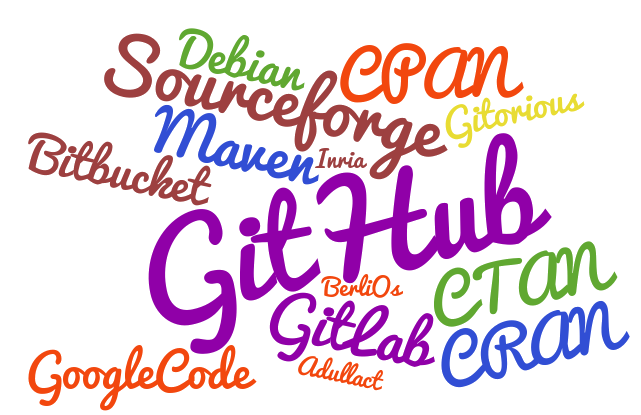
\includegraphics[width=.6\linewidth]{img/myriadsources}
    %                 \end{center}
    %                 \alert{find} and \alert{reference} all software source code
    %                 % \pause
    %             \end{block}
    %         \end{column}
    %         \begin{column}{.3\columnwidth}
    %             \begin{block}{Universal archive}
    %                 \begin{center}
    %                     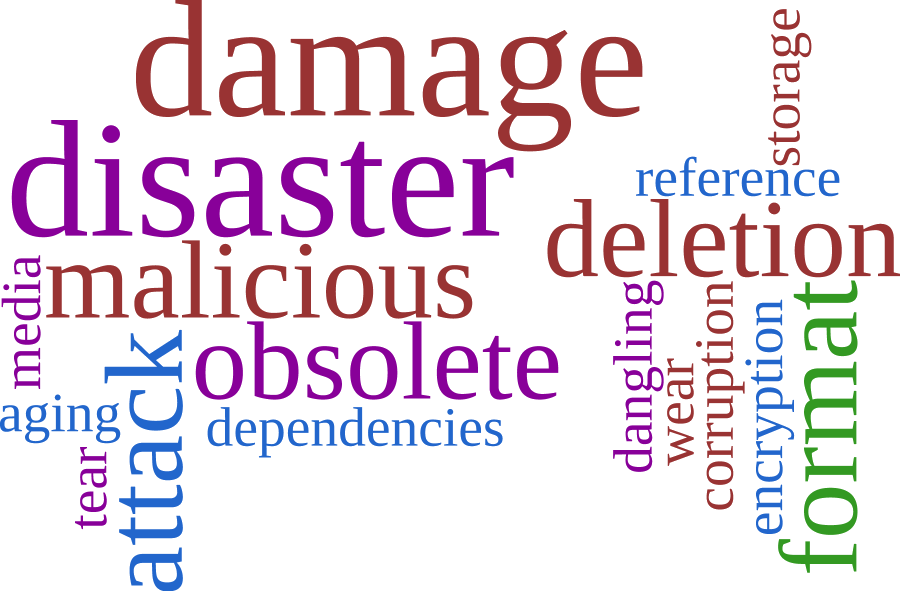
\includegraphics[width=.6\linewidth]{img/fragilecloud}
    %                 \end{center}
    %                 \alert{preserve} all software source code
    %                 % \pause
    %             \end{block}
    %         \end{column}
    %         \begin{column}{.3\columnwidth}
    %             \begin{block}{Research infrastructure}
    %                 \begin{center}
    %                     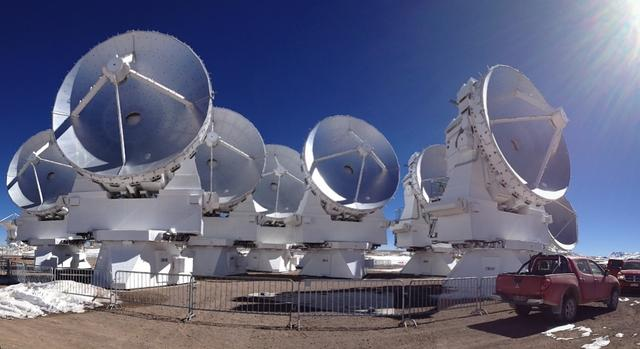
\includegraphics[width=.7\linewidth]{img/atacama-telescope}
    %                 \end{center}
    %                 \alert{enable analysis} of all software source code
    %             \end{block}
    %         \end{column}
    %     \end{columns}
    % \end{frame}

    % \begin{frame}
    %     \frametitle{Data flow}
    %     \begin{center}
    %         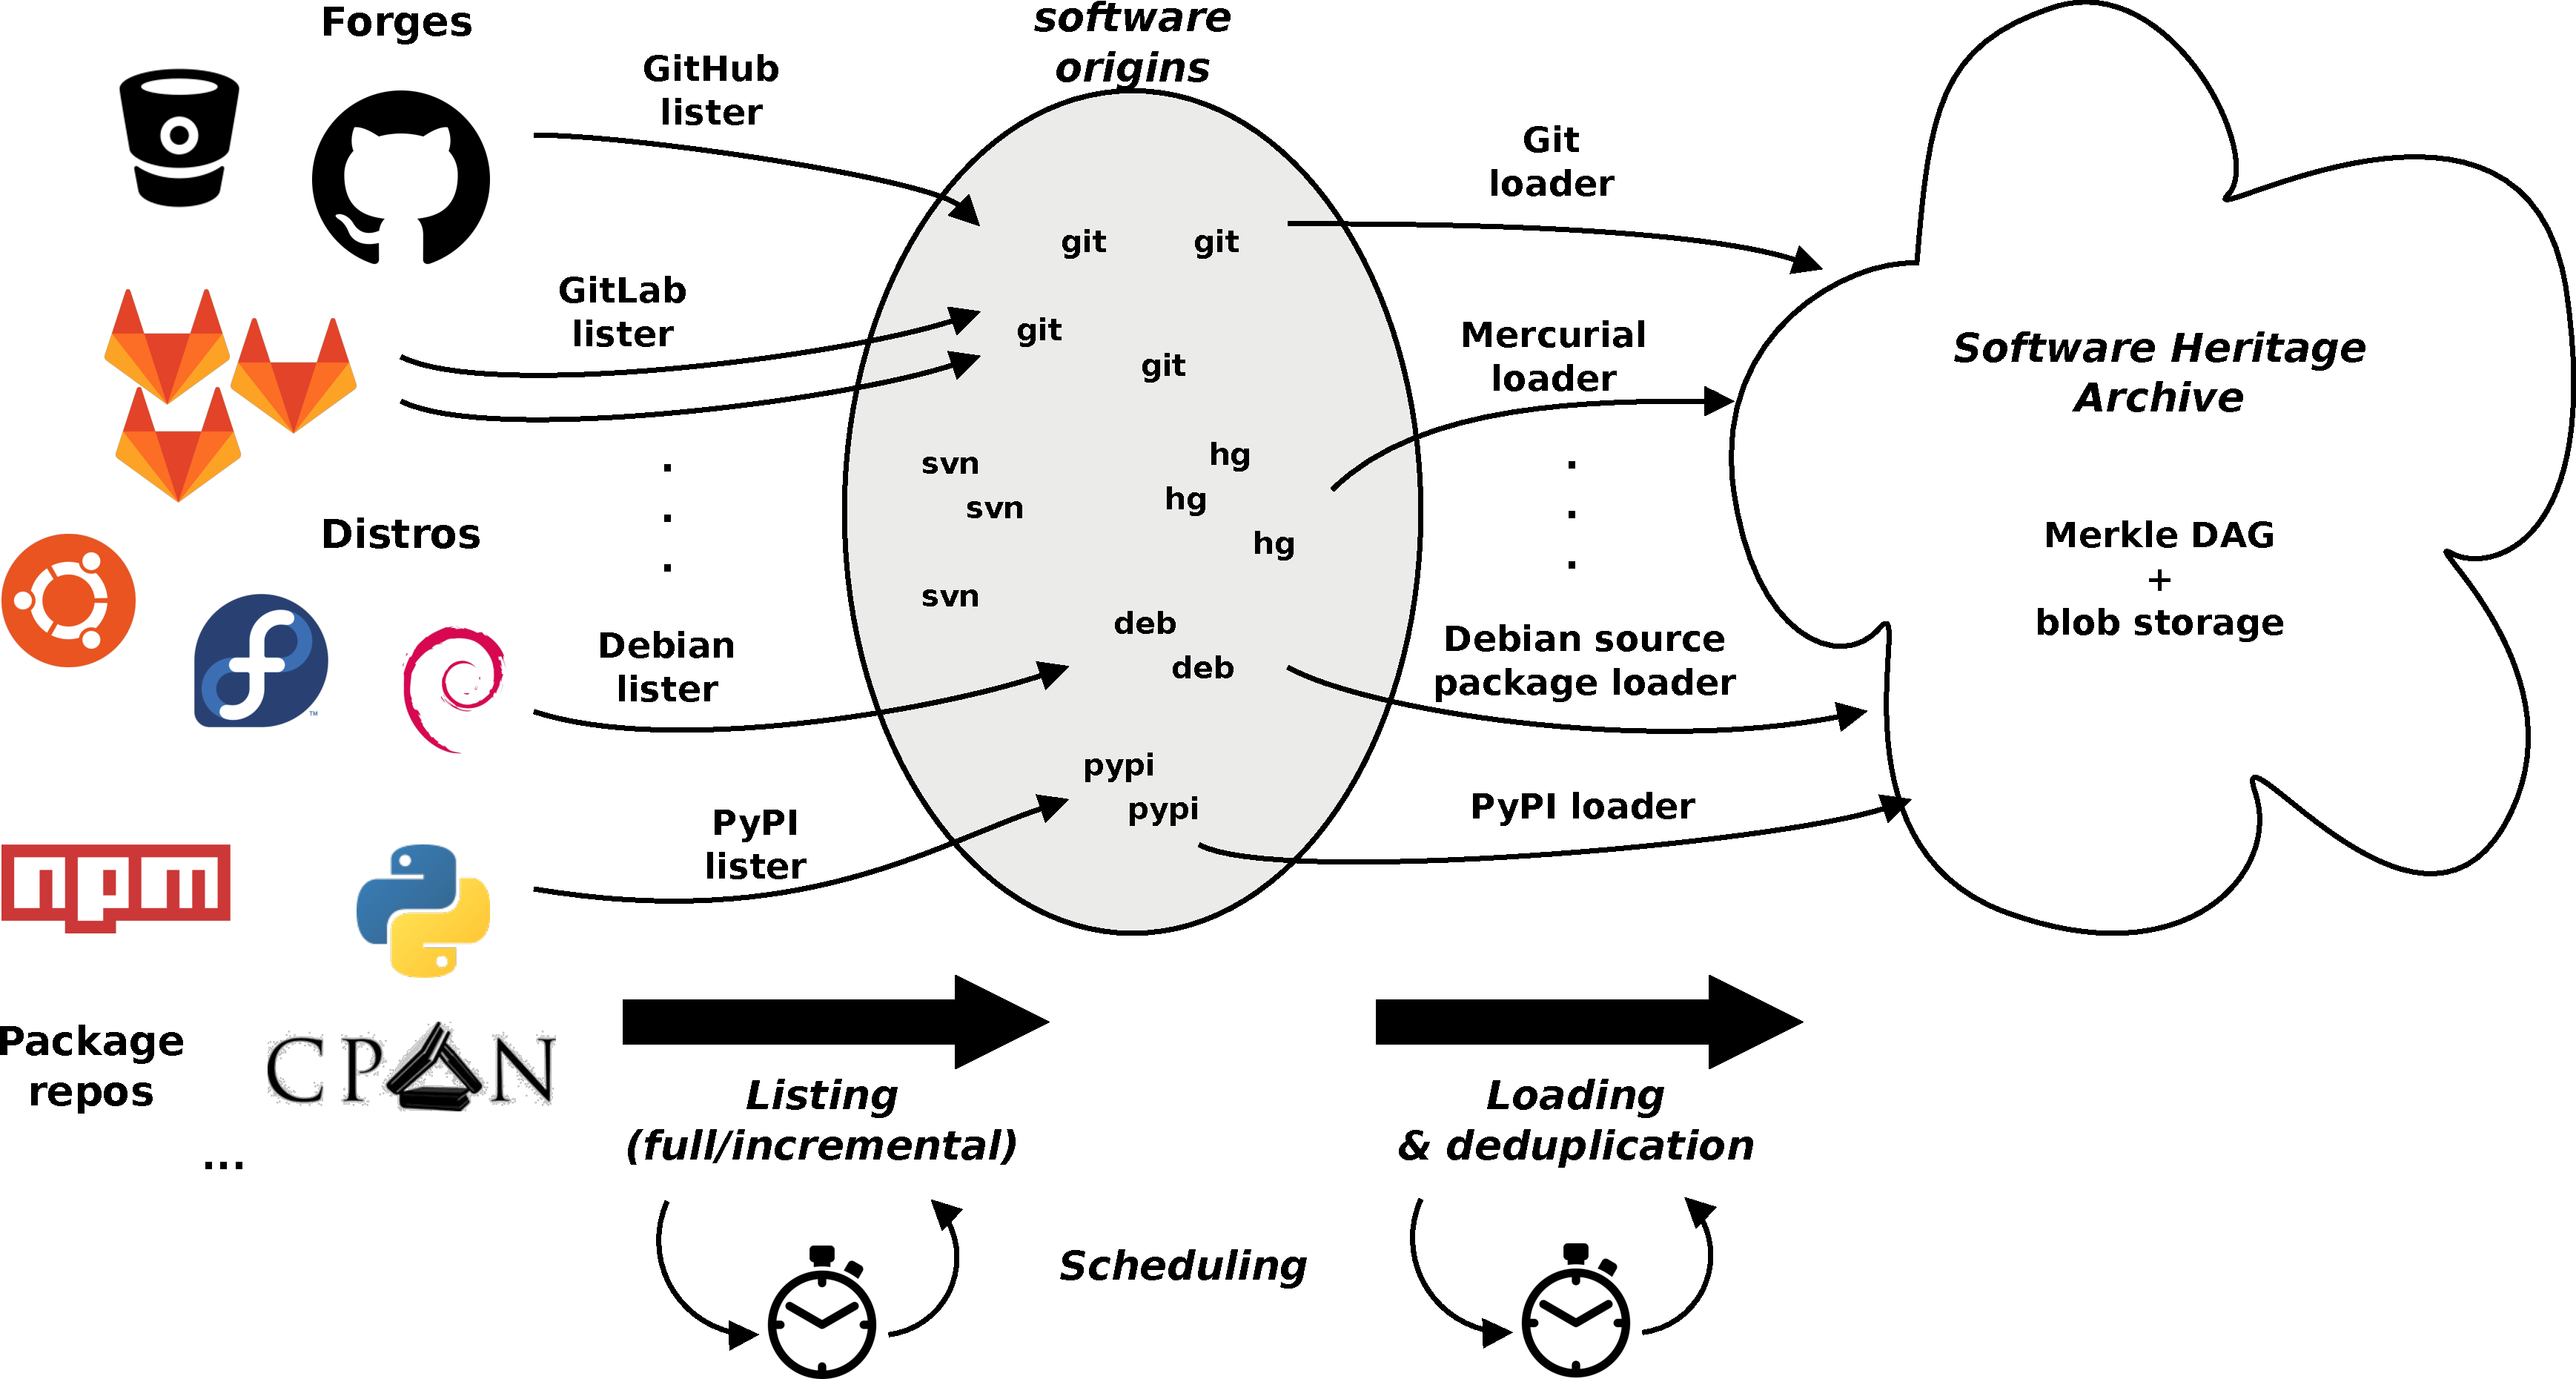
\includegraphics[width=0.9\textwidth]{img/swh-dataflow.pdf}
    %     \end{center}
    % \end{frame}

    \begin{frame}
        \frametitle{Corpus: The Software Heritage Archive ---
        archive.softwareheritage.org}

        \pdfpcnote{%
            As an approximation for this body of software development data, we
            use the Software Heritage archive, which is to my knowledge the
            largest and most exhaustive dataset of software development data
            available publicly.
            \\\\
            It contains more than 10 billion source files from more than 150
            million projects, which sums up to more than 900 TB on disk.
            \\\\
            It archives data from a variety of different places, collaborative
            development platforms like GitHub, Gitlab or Bitbucket, language
            package managers like NPM or PyPI or distribution packages like
            NixOS or Debian. This variety of sources is really interesting
            because it gives us a complete picture of software development in
            general, and not specific to a single platform.
        }

        \begin{block}{}
            \begin{itemize}
                \item We use the \textbf{Software Heritage archive} as our best
                    approximation of the entire corpus of public software
                    development.
                \item Largest public source code archive in the world (more
                    than 900 TB, growing daily).
            \end{itemize}
        \end{block}
        % TODO: update numbers?
        % \vspace{-1mm}
        \begin{center}
            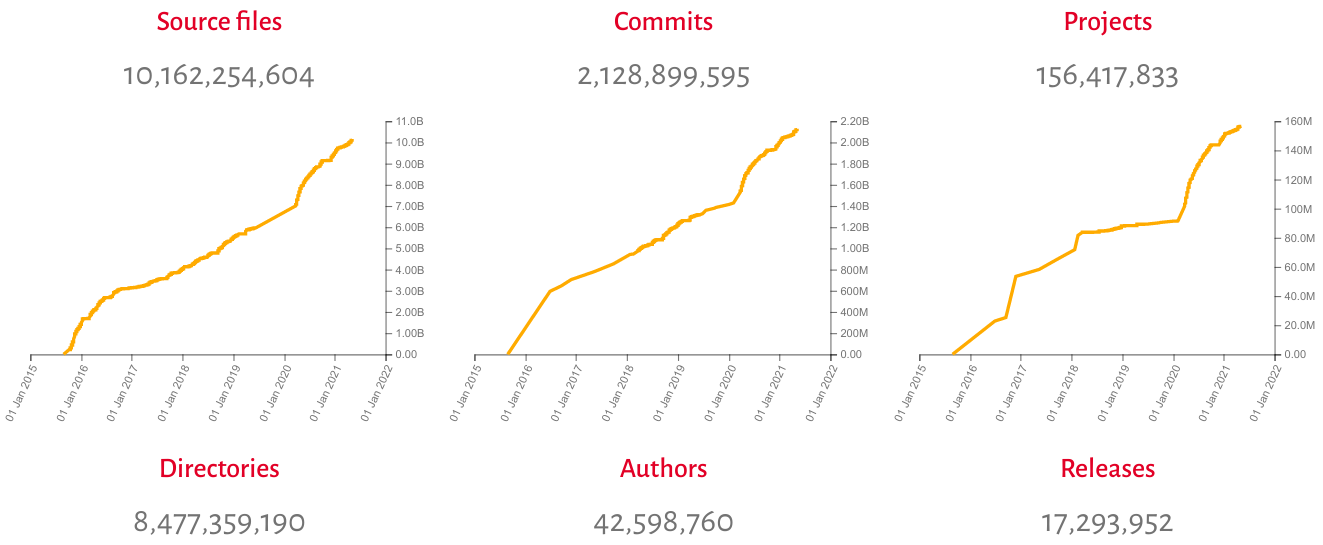
\includegraphics[trim=0 2cm 0 0, clip, width=0.7\linewidth]{img/archive-growth.png}
        \end{center}
        % \vspace{-2mm}
        \begin{center}
            \colorbox{white}{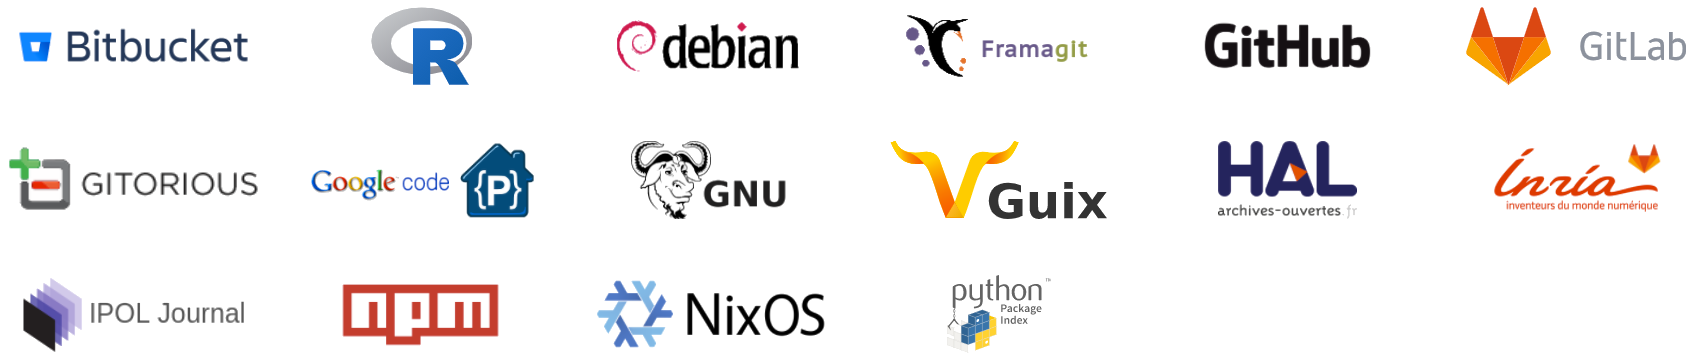
\includegraphics[width=0.7\linewidth]{img/archive-coverage.png}}
        \end{center}
        % \pause
        \vspace{-2mm}
        \begin{block}{}
            \begin{itemize}
                \item On disk: \textasciitilde{}750 TB (uncompressed)
                \item The largest public archive of source code in the world
                    (and growing!)
            \end{itemize}
        \end{block}
    \end{frame}

    \begin{frame}{Outline}
        \tableofcontents

        \pdfpcnote{%
            Here is the outline of this presentation.
            \\\\
            First I'm going to present a generic data model of the software
            development data that researchers might want to exploit.
            \\\\
            Then I'll discuss different ways we can make this data accessible
            for software mining at different scales.
            \\\\
            We will see that these approaches have some limitations. To address
            them, I'll introduce graph compression as a way to efficiently run
            analyses on this corpus.
            \\\\
            Finally I describe two empirical studies I performed on the graph
            of software development, one on the topology of the graph of
            software development, and another to identify software forks.
        }
    \end{frame}

    \section{Data Model}

    \begin{frame}
        \frametitle{A source code directory}

        \pdfpcnote{%
            At a fundamental level, the basic building block of software
            development is source code directories. Here is a very simple
            example of a program written in C.
            \\\\
            There are two types of objects here, source code files at the
            bottom, and the directories that organize them in a tree hierarchy.
            \\\\
            This code generally doesn't remain static, it evolves over time.
            It's really useful to keep track of this evolution.
        }

        \begin{columns}
            \column{.30\textwidth}
            \begin{figure}
                \begin{minipage}{\textwidth}
                \dirtree{%
                    .1 /.
                        .2 src.
                            .3 evalexpr.c.
                            .3 parser.
                                .4 ast.c.
                                .4 parser.c.
                                .4 lexer.c.
                        .2 tests.
                            .3 eval.c.
                            .3 operands.c.
                }
            \end{minipage}
            \end{figure}
            \column{.70\textwidth}
            \begin{figure}
                \centering
                \scalebox{0.9}{\begin{tikzpicture}[scale=2, font=\footnotesize]
	\begin{pgfonlayer}{nodelayer}
		\node [style=directory] (9) at (3, -2) {};
		\node [style=directory] (10) at (1, -2) {};
		\node [style=directory] (14) at (1.5, -3) {};
		\node [style=content] (16) at (1.5, -4) {};
		\node [style=content] (17) at (2.25, -4) {};
		\node [style=content] (18) at (0.75, -4) {};
		\node [style=content] (19) at (0, -3) {};
		\node [style=directory] (20) at (2, -1.5) {};
		\node [style=content] (21) at (2.5, -3) {};
		\node [style=content] (22) at (3.5, -3) {};
	\end{pgfonlayer}
	\begin{pgfonlayer}{edgelayer}
		\draw [style=arrow] (20) to node [above,sloped] {src} (10);
		\draw [style=arrow] (10) to node [above,sloped] {evalexpr.c} (19);
		\draw [style=arrow] (10) to node [above,sloped] {parser} (14);
		\draw [style=arrow] (14) to node [above,sloped] {ast.c} (16);
		\draw [style=arrow] (14) to node [above,sloped] {lexer.c} (17);
		\draw [style=arrow] (14) to node [above,sloped] {parser.c} (18);
		\draw [style=arrow] (20) to node [above,sloped] {tests} (9);
		\draw [style=arrow] (9) to node [above,sloped] {parser.c} (21);
		\draw [style=arrow] (9) to node [above,sloped] {operands.c} (22);
	\end{pgfonlayer}
\end{tikzpicture}
}
            \end{figure}
        \end{columns}
    \end{frame}

    \begin{frame}
        \frametitle{Revisions}
        \pdfpcnote{%
            For that, we introduce another type of object called revisions or
            commits. They form a chain that retains frozen past states of the
            source directory.
            \\\\
            Keeping track of how the codebase evolved is really useful to
            developers, because it allows them to quickly find where a bug
            was introduced and go back to a working state. It also allows
            them to retain institutional knowledge by keeping a memory
            of all the changes that were introduced over time.
        }

        % Parallel history
        \begin{block}{}
            \begin{itemize}
                \item \textbf{Revisions} (or ``commits'') keep track of
                    successive states of a source directory.
            \end{itemize}
        \end{block}
        \vfill
        \begin{figure}
            \centering
            \scalebox{0.8}{\begin{tikzpicture}[scale=1.5, font={\small}]
	\begin{pgfonlayer}{nodelayer}
		\node [style=directory] (10) at (2, -1.5) {};
		\node [style=directory] (14) at (2, -2.25) {};
		\node [style=content] (16) at (2, -3) {};
		\node [style=content] (17) at (2.5, -3) {};
		\node [style=content] (18) at (1.5, -3) {};
		\node [style=content] (19) at (1.25, -2.25) {};
		\node [style=directory] (20) at (2, -0.75) {};
		\node [style=revision, label={[align=center]\textbf{Second revision} \\ Add parser}] (23) at (2, 0) {};
		\node [style=revision, label={[align=center]\textbf{Third revision} \\ Add tests}] (24) at (5, 0) {};
		\node [style=directory] (25) at (5.5, -1.5) {};
		\node [style=directory] (26) at (4.5, -1.5) {};
		\node [style=directory] (27) at (4.5, -2.25) {};
		\node [style=content] (28) at (4.5, -3) {};
		\node [style=content] (29) at (5, -3) {};
		\node [style=content] (30) at (4, -3) {};
		\node [style=content] (31) at (3.75, -2.25) {};
		\node [style=directory] (32) at (5, -0.75) {};
		\node [style=content] (33) at (5.25, -2.25) {};
		\node [style=content] (34) at (5.75, -2.25) {};
		\node [style=revision, label={[align=center]\textbf{First revision} \\ Initial prototype}] (35) at (-1, 0) {};
		\node [style=directory] (36) at (-1, -0.75) {};
		\node [style=content] (37) at (-1, -1.5) {};
	\end{pgfonlayer}
	\begin{pgfonlayer}{edgelayer}
		\draw [style=arrow] (10) to (14);
		\draw [style=arrow] (14) to (16);
		\draw [style=arrow] (14) to (17);
		\draw [style=arrow] (20) to node [above, sloped] {\tiny src} (10);
		\draw [style=arrow] (10) to (19);
		\draw [style=arrow] (14) to (18);
		\draw [style=arrow] (23) to (20);
		\draw [style=arrow] (24) to (23);
		\draw [style=arrow] (26) to (27);
		\draw [style=arrow] (27) to (28);
		\draw [style=arrow] (27) to (29);
		\draw [style=arrow] (32) to node [above, sloped] {\tiny src} (26);
		\draw [style=arrow] (32) to node [above, sloped] {\tiny tests} (25);
		\draw [style=arrow] (26) to (31);
		\draw [style=arrow] (27) to (30);
		\draw [style=arrow] (25) to (33);
		\draw [style=arrow] (25) to (34);
		\draw [style=arrow] (24) to (32);
		\draw [style=arrow] (23) to (35);
		\draw [style=arrow] (35) to (36);
		\draw [style=arrow] (36) to (37);
	\end{pgfonlayer}
\end{tikzpicture}
}
        \end{figure}
    \end{frame}

    \begin{frame}
        \frametitle{Branches}
        \pdfpcnote{%
            An advantage of this design is that it allows developers to work in
            parallel, on separate features. For that, they can work on branches
            that they ``merge'' back when they want to integrate their work to
            a mainline.
        }

        \begin{block}{}
            Developers can use ``branches'' to work on different features
            simultaneously.
        \end{block}
        \vfill
        % TODO: add a time arrow
        \begin{figure}
            \centering
            \scalebox{0.8}{\begin{tikzpicture}
	\begin{pgfonlayer}{nodelayer}
		\node [style=revision] (0) at (0, 0) {};
		\node [style=revision, label={[align=center]below:Branching\\revision}] (1) at (2, 0) {};
		\node [style=revision] (2) at (4, 0) {};
		\node [style=revision] (3) at (3, 1) {};
		\node [style=revision] (4) at (4.75, 1) {};
		\node [style=revision] (5) at (6, 0) {};
		\node [style=revision, label={[align=center]below:Merge\\revision}] (6) at (8, 0) {};
		\node [style=revision] (7) at (6.5, 1) {};
		\node [style=revision] (8) at (9.5, 0) {};
	\end{pgfonlayer}
	\begin{pgfonlayer}{edgelayer}
		\draw [style=arrow] (1) to (0);
		\draw [style=arrow] (3) to (1);
		\draw [style=arrow] (4) to (3);
		\draw [style=arrow] (7) to (4);
		\draw [style=arrow] (6) to (7);
		\draw [style=arrow] (2) to (1);
		\draw [style=arrow] (5) to (2);
		\draw [style=arrow] (6) to (5);
		\draw [style=arrow] (8) to (6);
	\end{pgfonlayer}
\end{tikzpicture}
}
        \end{figure}
    \end{frame}

    % \begin{frame}
    %     \frametitle{Branches}
    %     \begin{block}{}
    %         \begin{itemize}
    %             \item \textbf{Branches} are dynamic pointers to revisions,
    %                 using mnemonic names to keep track of their purpose.
    %             \item Branch pointers move when more revisions are added to the
    %                 branch.
    %         \end{itemize}
    %     \end{block}
    %     % TODO: animate
    %     \vfill
    %     \begin{figure}
    %         \centering
    %         \scalebox{0.8}{\begin{tikzpicture}
	\begin{pgfonlayer}{nodelayer}
		\node [style=revision] (0) at (0, 0) {};
		\node [style=revision] (1) at (2, 0) {};
		\node [style=revision] (2) at (4, 0) {};
		\node [style=revision] (3) at (6, 0) {};
		\node [style=revision] (4) at (8, 0) {};
		\node [style=revision] (5) at (3, 1) {};
		\node [style=revision] (6) at (5, 1) {};
		\node [style=revision] (7) at (5, -1) {};
		\node [style=revision] (8) at (7, -1) {};
		\node [style=branch] (9) at (5, 2.25) {feature-parser};
		\node [style=branch] (10) at (8, 2.25) {main};
		\node [style=branch] (11) at (9, 1) {test-ci};
		\node [style=revision] (12) at (9, -1) {};
	\end{pgfonlayer}
	\begin{pgfonlayer}{edgelayer}
		\draw [style=arrow] (1) to (0);
		\draw [style=arrow] (2) to (1);
		\draw [style=arrow] (3) to (2);
		\draw [style=arrow] (4) to (3);
		\draw [style=arrow] (5) to (1);
		\draw [style=arrow] (6) to (5);
		\draw [style=arrow] (7) to (2);
		\draw [style=arrow] (8) to (7);
		\draw [style=dashed arrow] (9) to (6);
		\draw [style=dashed arrow] (10) to (4);
		\draw [style=dashed arrow] (11) to (12);
		\draw [style=arrow] (12) to (8);
	\end{pgfonlayer}
\end{tikzpicture}
}
    %     \end{figure}
    % \end{frame}

    % \begin{frame}
    %     \frametitle{Releases}
    %     \begin{block}{}
    %         \begin{itemize}
    %             \item \textbf{Releases} (or ``tags'') point to specific
    %                 milestones in the development history.
    %             \item Their names usually represent the software versions.
    %         \end{itemize}
    %     \end{block}
    %     % TODO: animate
    %     \vfill
    %     \begin{figure}
    %         \centering
    %         \scalebox{0.8}{\begin{tikzpicture}
	\begin{pgfonlayer}{nodelayer}
		\node [style=revision] (0) at (0, 0) {};
		\node [style=revision] (1) at (2, 0) {};
		\node [style=revision] (2) at (4, 0) {};
		\node [style=revision] (3) at (6, 0) {};
		\node [style=revision] (4) at (8, 0) {};
		\node [style=revision] (7) at (3, -1) {};
		\node [style=revision] (8) at (5, -1) {};
		\node [style=branch] (10) at (10, 2) {main};
		\node [style=revision] (12) at (7, -1) {};
		\node [style=revision] (13) at (10, 0) {};
		\node [style=revision] (14) at (6, -2) {};
		\node [style=revision] (15) at (8, -2) {};
		\node [style=release, label={\textbf{v2.0}}] (16) at (8, 2) {};
		\node [style=release, label={\textbf{v1.0}}] (17) at (4, 2) {};
	\end{pgfonlayer}
	\begin{pgfonlayer}{edgelayer}
		\draw [style=arrow] (1) to (0);
		\draw [style=arrow] (2) to (1);
		\draw [style=arrow] (3) to (2);
		\draw [style=arrow] (4) to (3);
		\draw [style=arrow] (8) to (7);
		\draw [style=arrow] (12) to (8);
		\draw [style=arrow] (4) to (12);
		\draw [style=arrow] (7) to (1);
		\draw [style=dashed arrow] (10) to (13);
		\draw [style=arrow] (13) to (4);
		\draw [style=arrow] (14) to (8);
		\draw [style=arrow] (15) to (14);
		\draw [style=dashed arrow] (16) to (4);
		\draw [style=dashed arrow] (17) to (2);
	\end{pgfonlayer}
\end{tikzpicture}
}
    %     \end{figure}
    % \end{frame}

    % \begin{frame}
    %     \frametitle{Deduplication}
    %     \begin{block}{}
    %         \begin{itemize}
    %             \item Lots of frozen states $\Rightarrow$ lots of copies of
    %                 objects
    %             \item Most objects stay identical from one revision to another
    %             \pause
    %             \item We can identify \& deduplicate them with
    %                 \textbf{cryptographic hash functions}.
    %         \end{itemize}
    %     \end{block}
    %     \vfill
    %     \begin{figure}
    %         \centering
    %         \scalebox{0.8}{\begin{tikzpicture}
    \node [
        shape=rectangle, draw=black, align=left, font=\tiny,
        label={[above]Input text}
    ] (input) at (0, 0)
        {%
            L'argoumante était églomatique et s'impliquait \\
            beaucoup plus qu'à l'exparité. Le plus déjà se \\
            plussissait. Plus qu'à l'exparité s'étrangent et se \\
            consument les pregmes endiablés de la légume.
    };

    \node [
        shape=ellipse, draw=black, align=left, fill=cyan!25,
        label={[above,align=center]Cryptographic \\ hash function}
    ] (hash) at (5.5, 0) {SHA-256};

    \node [
        shape=rectangle, draw=black, align=center, font=\footnotesize,
        label={[above]Result hash}
    ] (output) at (10, 0) {%
        % \texttt{7a50e30ada8f09b2}%
        % \texttt{24d348d314de4c09} \\
        % \texttt{ae0ebcb443334442}%
        % \texttt{70cc832ebfc6bc0c}

        \texttt{7a50e30ada8f09b224d34} \\
        \texttt{8d314de4c09ae0ebcb443} \\
        \texttt{33444270cc832ebfc6bc0c}
    };

    \draw[->, >=Stealth] (input) to (hash);
    \draw[->, >=Stealth] (hash) to (output);
\end{tikzpicture}
}
    %     \end{figure}
    %     \begin{block}{Cryptographic hash functions (SHA-1, SHA-256, BLAKE2, …)}
    %         \begin{itemize}
    %             \item Associates an arbitrary input with a
    %                 \emph{unique\footnote{Terms and conditions apply.}
    %                 identifier} called a \textbf{hash}
    %             \item Check if two objects are identical in O(1).
    %         \end{itemize}
    %     \end{block}
    % \end{frame}

    % \begin{frame}
    %     \frametitle{Deduplicating files}
    %     \begin{block}{}
    %         \begin{itemize}
    %             \item VCSs identify each file via their unique hash
    %             \item Identical files are \emph{deduplicated} (= shared) from
    %                 one revision to another.
    %         \end{itemize}
    %     \end{block}
    %     % TODO: animate
    %     \vfill
    %     \begin{figure}
    %         \centering
    %         \scalebox{0.8}{\begin{tikzpicture}[scale=1.5, font={\small}]
	\begin{pgfonlayer}{nodelayer}
		\node [style=directory] (10) at (2, -1.5) {};
		\node [style=directory] (14) at (2, -2.25) {};
		\node [style=content] (16) at (2, -3.5) {C};
		\node [style=content] (17) at (2.5, -3.5) {D};
		\node [style=content] (18) at (1.5, -3.5) {B};
		\node [style=content, fill=white, dotted] (19) at (1.25, -2.25) {A};
		\node [style=directory] (20) at (2, -0.75) {};
		\node [style=revision] (23) at (2, 0) {};
		\node [style=revision] (24) at (5, 0) {};
		\node [style=directory] (25) at (5.5, -1.5) {};
		\node [style=directory] (26) at (4.5, -1.5) {};
		\node [style=directory] (27) at (4.5, -2.25) {};
		\node [style=content, fill=white, dotted] (28) at (4.5, -3.5) {C};
		\node [style=content, fill=white, dotted] (29) at (5, -3.5) {D};
		\node [style=content, fill=white, dotted] (30) at (4, -3.5) {B};
		\node [style=content, fill=white, dotted] (31) at (3.75, -2.25) {A};
		\node [style=directory] (32) at (5, -0.75) {};
		\node [style=content] (33) at (5.25, -2.25) {E};
		\node [style=content] (34) at (5.75, -2.25) {F};
		\node [style=revision] (35) at (-1, 0) {};
		\node [style=directory] (36) at (-1, -0.75) {};
		\node [style=content] (37) at (-1, -1.5) {A};
	\end{pgfonlayer}
	\begin{pgfonlayer}{edgelayer}
		\draw [style=arrow] (10) to (14);
		\draw [style=arrow] (14) to (16);
		\draw [style=arrow] (14) to (17);
		\draw [style=arrow] (20) to node [above, sloped] {\tiny src} (10);
		\draw [style=dashed arrow, dotted] (10) to (19);
		\draw [style=arrow] (14) to (18);
		\draw [style=arrow] (23) to (20);
		\draw [style=arrow] (24) to (23);
		\draw [style=arrow] (26) to (27);
		\draw [style=dashed arrow, dotted] (27) to (28);
		\draw [style=dashed arrow, dotted] (27) to (29);
		\draw [style=arrow] (32) to node [above, sloped] {\tiny src} (26);
		\draw [style=arrow] (32) to node [above, sloped] {\tiny tests} (25);
		\draw [style=dashed arrow, dotted] (26) to (31);
		\draw [style=dashed arrow, dotted] (27) to (30);
		\draw [style=arrow] (25) to (33);
		\draw [style=arrow] (25) to (34);
		\draw [style=arrow] (24) to (32);
		\draw [style=arrow] (23) to (35);
		\draw [style=arrow] (35) to (36);
		\draw [style=arrow] (36) to (37);
		\draw [style=red arrow, bend left=15] (10) to (37);
		\draw [style=red arrow, bend left=15, looseness=0.75] (26) to (37);
		\draw [style=red arrow, in=-300, out=-135, looseness=0.75] (27) to (18);
		\draw [style=red arrow, in=75, out=-135, looseness=0.75] (27) to (16);
		\draw [style=red arrow, in=75, out=-135] (27) to (17);
	\end{pgfonlayer}
\end{tikzpicture}
}
    %     \end{figure}
    % \end{frame}

    \begin{frame}
        \frametitle{Deduplication}
        \pdfpcnote{%
            Copying these states from one revision to another will duplicate a
            lot of identical objects, like files and directories that weren't
            modified in a given revision. Instead of just storing copies, we
            can identify these duplicate nodes using cryptographic hash
            functions.
            \\\\
            We can attribute a unique fixed-length identifier to any given
            object in the graph by recursively computing these hash functions
            on their entire subtrees. We then store them as single nodes in the
            graph, so a unique directory will only be present once in this
            graph even if a lot of revisions or other directories point towards
            it.
        }
        \begin{block}{}
            \begin{itemize}
                \item Instead of copying the nodes between each revision, we
                    can identify \& deduplicate them with \textbf{cryptographic
                    hash functions} (e.g., SHA-1)
                \item Each object is identified by a unique identifier
                    (``hash'') computed from its entire subtree
            \end{itemize}
        \end{block}
        % TODO: animate
        \vfill
        \begin{figure}
            \centering
            \scalebox{0.8}{\begin{tikzpicture}[scale=1.5, font={\small}]
	\begin{pgfonlayer}{nodelayer}
		\node [style=directory] (10) at (2, -1.5) {3};
		\node [style=directory] (14) at (2, -2.25) {4};
		\node [style=content] (16) at (2, -3.5) {C};
		\node [style=content] (17) at (2.5, -3.5) {D};
		\node [style=content] (18) at (1.5, -3.5) {B};
		\node [style=content, fill=white, dotted] (19) at (1.25, -2.25) {A};
		\node [style=directory] (20) at (2, -0.75) {2};
		\node [style=revision] (23) at (2, 0) {};
		\node [style=revision] (24) at (4.25, 0) {};
		\node [style=directory] (25) at (4.75, -1.5) {6};
		\node [style=directory, fill=white, dotted] (26) at (3.75, -1.5) {3};
		\node [style=directory, fill=white, dotted] (27) at (3.75, -2.25) {4};
		\node [style=content, fill=white, dotted] (28) at (3.75, -3.5) {C};
		\node [style=content, fill=white, dotted] (29) at (4.25, -3.5) {D};
		\node [style=content, fill=white, dotted] (30) at (3.25, -3.5) {B};
		\node [style=content, fill=white, dotted] (31) at (3, -2.25) {A};
		\node [style=directory] (32) at (4.25, -0.75) {5};
		\node [style=content] (33) at (4.5, -2.25) {E};
		\node [style=content] (34) at (5, -2.25) {F};
		\node [style=revision] (35) at (0.25, 0) {};
		\node [style=directory] (36) at (0.25, -0.75) {1};
		\node [style=content] (37) at (0.25, -2.25) {A};
	\end{pgfonlayer}
	\begin{pgfonlayer}{edgelayer}
		\draw [style=arrow] (10) to (14);
		\draw [style=arrow] (14) to (16);
		\draw [style=arrow] (14) to (17);
		\draw [style=arrow] (20) to node [above, sloped] {\tiny src} (10);
		\draw [style=dashed arrow, dotted] (10) to (19);
		\draw [style=arrow] (14) to (18);
		\draw [style=arrow] (23) to (20);
		\draw [style=arrow] (24) to (23);
		\draw [style=dashed arrow, dotted] (26) to (27);
		\draw [style=dashed arrow, dotted] (27) to (28);
		\draw [style=dashed arrow, dotted] (27) to (29);
		\draw [style=dashed arrow, dotted] (32) to node [above, sloped, color={black!60}] {\tiny src} (26);
		\draw [style=arrow] (32) to node [above, sloped] {\tiny tests} (25);
		\draw [style=dashed arrow, dotted] (26) to (31);
		\draw [style=dashed arrow, dotted] (27) to (30);
		\draw [style=arrow] (25) to (33);
		\draw [style=arrow] (25) to (34);
		\draw [style=arrow] (24) to (32);
		\draw [style=arrow] (23) to (35);
		\draw [style=arrow] (35) to (36);
		\draw [style=arrow] (36) to (37);
		\draw [style=red arrow, bend right=15] (10) to (37);
		\draw [style=red arrow] (32) to node [above, sloped, color={red!70!black}] {\tiny src} (10);
	\end{pgfonlayer}
\end{tikzpicture}
}
        \end{figure}
    \end{frame}

    % \begin{frame}
    %     \frametitle{Merkle DAG}
    %     \begin{block}{}
    %         \begin{itemize}
    %             \item Changing a single object only requires
    %                 $O(h)$ new nodes
    %         \end{itemize}
    %     \end{block}
    %     \vfill
    %     \begin{figure}
    %         \centering
    %         \scalebox{0.8}{\begin{tikzpicture}[scale=1.5, font={\small}]
	\begin{pgfonlayer}{nodelayer}
		\node [style=directory] (10) at (1.5, -1.5) {};
		\node [style=directory] (14) at (1.5, -2.25) {};
		\node [style=content] (16) at (1.25, -3.25) {C};
		\node [style=content] (17) at (1.75, -3.25) {D};
		\node [style=directory] (20) at (2, -0.75) {};
		\node [style=revision] (23) at (2, 0) {};
		\node [style=revision] (24) at (6, 0) {};
		\node [style=directory] (25) at (2.5, -1.5) {};
		\node [style=directory] (29) at (2.5, -2.25) {};
		\node [style=directory] (30) at (3.25, -2.25) {};
		\node [style=content] (31) at (2.75, -3.25) {F};
		\node [style=content] (32) at (3.25, -3.25) {G};
		\node [style=content] (33) at (3.75, -3.25) {H};
		\node [style=directory] (37) at (6, -0.75) {};
		\node [style=directory] (38) at (6, -1.5) {};
		\node [style=directory] (39) at (6, -2.25) {};
		\node [style=content] (40) at (6, -3.25) {H'};
		\node [style=directory] (42) at (0.75, -2.25) {};
		\node [style=content] (43) at (2.25, -3.25) {E};
		\node [style=content] (44) at (0.75, -3.25) {B};
		\node [style=content] (45) at (0.25, -3.25) {A};
	\end{pgfonlayer}
	\begin{pgfonlayer}{edgelayer}
		\draw [style=arrow] (10) to (14);
		\draw [style=arrow] (14) to (16);
		\draw [style=arrow] (14) to (17);
		\draw [style=arrow] (20) to (10);
		\draw [style=arrow] (24) to (23);
		\draw [style=arrow] (25) to (29);
		\draw [style=arrow] (29) to (31);
		\draw [style=arrow] (30) to (32);
		\draw [style=arrow] (10) to (42);
		\draw [style=arrow] (42) to (44);
		\draw [style=arrow] (42) to (45);
		\draw [style=arrow] (29) to (43);
		\draw [style=arrow, in=-315, out=-150, looseness=1.25] (38) to (29);
		\draw [style=arrow, in=-300, out=-150, looseness=1.25] (39) to (32);
		\draw [style=arrow, in=-330, out=-150, looseness=1.25] (37) to (10);
		\draw [style=red arrow] (20) to (25);
		\draw [style=red arrow] (25) to (30);
		\draw [style=red arrow] (23) to (20);
		\draw [style=red arrow] (30) to (33);
		\draw [style=red arrow] (24) to (37);
		\draw [style=red arrow] (37) to (38);
		\draw [style=red arrow] (38) to (39);
		\draw [style=red arrow] (39) to (40);
		\draw [decorate, decoration={brace,raise=20pt,amplitude=10pt}] (24) to node [right=35pt, style=none] {$h$} (40);
	\end{pgfonlayer}
\end{tikzpicture}
}
    %     \end{figure}
    % \end{frame}

    \begin{frame}
        \frametitle{Consolidation in a single archive}
        \pdfpcnote{%
            The Software Heritage data models extends this idea of
            deduplication of identical objects, but it applies it to the entire
            corpus of software data.
            Basically, all the repositories are consolidated into a single
            archive, and then the objects contained in these repositories are
            deduplicated, but across all the repositories at once. If a file or
            a directory was copied across multiple repositories, they will
            still only be stored once in the archive.
            \\\\
            This is a really interesting data model, because in effect it
            materializes a giant graph which gives us a global, unified view of
            all the software development artifacts from VCS that software
            mining researchers might want to analyze. It's like a map of the
            stars of all the software data; we can directly see how code is
            reused across repos through the relationships between objects.
            \\\\
            One way to imagine it is to visualize a single giant Git repository
            with all the code in the world.
        }

        \begin{columns}
            \column{.50\textwidth}
            \begin{block}{}
                \begin{itemize}
                    \item In Software Heritage, \emph{all} the repositories are
                        consolidated into a single archive
                    \item Software artifacts are deduplicated \emph{across
                        different repositories}
                    \item The result is a single graph providing a
                        \textbf{global, unified view} on \textbf{all the
                        software development artifacts} from version control
                        systems
                    \item Helpful analogy: like a single Git repository but
                        with all the public code in the world.
                \end{itemize}
            \end{block}
            \column{.50\textwidth}
            \begin{figure}
                \centering
                \scalebox{0.4}{\begin{tikzpicture}[scale=1.3, font={\tiny}, {every node/.style}={scale=1}]
	\begin{pgfonlayer}{nodelayer}
		\node [style=directory] (10) at (2, -3.5) {3};
		\node [style=content] (14) at (2, -4.25) {B};
		\node [style=directory] (20) at (1.5, -2.75) {2};
		\node [style=revision] (23) at (1.5, -2) {$\beta$};
		\node [style=revision] (24) at (2.5, -2) {$\gamma$};
		\node [style=directory] (25) at (3, -3.5) {6};
		\node [style=directory] (32) at (2.5, -2.75) {5};
		\node [style=content] (33) at (2.75, -4.25) {C};
		\node [style=content] (34) at (3.5, -4.25) {D};
		\node [style=revision] (35) at (0.5, -2) {$\alpha$};
		\node [style=directory] (36) at (0.5, -2.75) {1};
		\node [style=content] (37) at (1.25, -4.25) {A};
		\node [style=none] (38) at (0, 0) {};
		\node [style=none] (39) at (4, 0) {};
		\node [style=none] (40) at (4, -4.75) {};
		\node [style=none] (41) at (0, -4.75) {};
		\node [style=release] (42) at (2.75, -1.25) {y};
		\node [style=directory] (43) at (2, -9.25) {3};
		\node [style=content] (44) at (2, -10) {B};
		\node [style=directory] (48) at (1.5, -8.5) {2};
		\node [style=revision] (49) at (1.5, -7.75) {$\beta$};
		\node [style=revision] (50) at (2.5, -7.75) {$\gamma'$};
		\node [style=directory] (51) at (3, -9.25) {6'};
		\node [style=directory] (52) at (2.5, -8.5) {5'};
		\node [style=content] (53) at (2.75, -10) {C};
		\node [style=content] (54) at (3.5, -10) {D'};
		\node [style=revision] (55) at (0.5, -7.75) {$\alpha$};
		\node [style=directory] (56) at (0.5, -8.5) {1};
		\node [style=content] (57) at (1.25, -10) {A};
		\node [style=none] (58) at (0, -5.75) {};
		\node [style=none] (59) at (4, -5.75) {};
		\node [style=none] (60) at (4, -10.5) {};
		\node [style=none] (61) at (0, -10.5) {};
		\node [style=release] (62) at (2.75, -7) {y'};
		\node [style=release] (63) at (1.5, -1.25) {x};
		\node [style=release] (64) at (1.5, -7) {x};
		\node [style=directory] (65) at (8.25, -6.5) {3};
		\node [style=content] (66) at (8.25, -7.25) {B};
		\node [style=directory] (70) at (7.75, -5.75) {2};
		\node [style=revision] (71) at (7.75, -5) {$\beta$};
		\node [style=revision] (72) at (8.75, -4.25) {$\gamma$};
		\node [style=directory] (73) at (9.25, -6.5) {6};
		\node [style=directory] (74) at (8.75, -5.75) {5};
		\node [style=content] (75) at (9, -7.25) {C};
		\node [style=content] (76) at (9.75, -7.25) {D};
		\node [style=revision] (77) at (6.75, -5) {$\alpha$};
		\node [style=directory] (78) at (6.75, -5.75) {1};
		\node [style=content] (79) at (7.5, -7.25) {A};
		\node [style=release] (80) at (8.75, -3.25) {y};
		\node [style=release] (81) at (7.75, -4.25) {x};
		\node [style=revision] (82) at (10, -5) {$\gamma'$};
		\node [style=release] (83) at (10, -3.25) {y'};
		\node [style=directory] (84) at (10, -5.75) {5'};
		\node [style=directory] (85) at (10.25, -6.5) {6'};
		\node [style=content] (87) at (10.75, -7.25) {D'};
		\node [style=none] (88) at (6, -1.75) {};
		\node [style=none] (89) at (11.5, -1.75) {};
		\node [style=none] (90) at (11.5, -8) {};
		\node [style=none] (91) at (6, -8) {};
		\node [style=snapshot] (92) at (2, -6.25) {SNP-2};
		\node [style=snapshot] (93) at (2, -0.5) {SNP-1};
		\node [style=snapshot] (94) at (7, -2.25) {SNP-1};
		\node [style=snapshot] (95) at (9, -2.25) {SNP-2};
		\node [style=none] (96) at (4, -2.5) {};
		\node [style=none] (97) at (4, -8.25) {};
		\node [style=none] (98) at (6, -4) {};
		\node [style=none] (99) at (6, -6) {};
		\node [style=none] (100) at (5, -5.25) {\normalsize \emph{Ingestion}};
	\end{pgfonlayer}
	\begin{pgfonlayer}{edgelayer}
		\draw [style=arrow] (10) to (14);
		\draw [style=arrow] (20) to (10);
		\draw [style=arrow] (23) to (20);
		\draw [style=arrow] (24) to (23);
		\draw [style=arrow] (32) to (25);
		\draw [style=arrow] (25) to (33);
		\draw [style=arrow] (25) to (34);
		\draw [style=arrow] (24) to (32);
		\draw [style=arrow] (23) to (35);
		\draw [style=arrow] (35) to (36);
		\draw [style=arrow] (36) to (37);
		\draw [style=arrow] (10) to (37);
		\draw [style=arrow] (32) to (10);
		\draw (38.center) to (41.center);
		\draw (41.center) to (40.center);
		\draw [in=270, out=90] (40.center) to (39.center);
		\draw (39.center) to node [above, sloped] {\normalsize \textbf{Repository 1}} (38.center);
		\draw [style=arrow] (42) to (24);
		\draw [style=arrow] (43) to (44);
		\draw [style=arrow] (48) to (43);
		\draw [style=arrow] (49) to (48);
		\draw [style=arrow] (50) to (49);
		\draw [style=arrow] (52) to (51);
		\draw [style=arrow] (51) to (53);
		\draw [style=arrow] (51) to (54);
		\draw [style=arrow] (50) to (52);
		\draw [style=arrow] (49) to (55);
		\draw [style=arrow] (55) to (56);
		\draw [style=arrow] (56) to (57);
		\draw [style=arrow] (43) to (57);
		\draw [style=arrow] (52) to (43);
		\draw (58.center) to (61.center);
		\draw (61.center) to (60.center);
		\draw (60.center) to (59.center);
		\draw (59.center) to node [above, sloped] {\normalsize \textbf{Repository 2}} (58.center);
		\draw [style=arrow] (63) to (23);
		\draw [style=arrow] (64) to (49);
		\draw [style=arrow] (62) to (50);
		\draw [style=arrow] (65) to (66);
		\draw [style=arrow] (70) to (65);
		\draw [style=arrow] (71) to (70);
		\draw [style=arrow] (72) to (71);
		\draw [style=arrow] (74) to (73);
		\draw [style=arrow] (73) to (75);
		\draw [style=arrow] (73) to (76);
		\draw [style=arrow] (72) to (74);
		\draw [style=arrow] (71) to (77);
		\draw [style=arrow] (77) to (78);
		\draw [style=arrow] (78) to (79);
		\draw [style=arrow] (65) to (79);
		\draw [style=arrow] (74) to (65);
		\draw [style=arrow] (80) to (72);
		\draw [style=arrow] (81) to (71);
		\draw [style=arrow] (83) to (82);
		\draw [style=arrow] (82) to (71);
		\draw [style=arrow] (85) to (87);
		\draw [style=arrow] (82) to (84);
		\draw [style=arrow] (84) to (85);
		\draw [style=arrow, bend right=15] (85) to (75);
		\draw (88.center) to (91.center);
		\draw (91.center) to (90.center);
		\draw (90.center) to (89.center);
		\draw (88.center) to node [above, sloped] {\normalsize \textbf{Software Heritage Merkle DAG}} (89.center);
		\draw [style=arrow] (93) to (63);
		\draw [style=arrow] (93) to (42);
		\draw [style=arrow] (92) to (64);
		\draw [style=arrow] (92) to (62);
		\draw [style=arrow] (94) to (81);
		\draw [style=arrow, in=150, out=-30] (94) to (80);
		\draw [style=arrow] (93) to (24);
		\draw [style=arrow] (92) to (50);
		\draw [style=arrow] (94) to (72);
		\draw [style=arrow, bend right=15] (95) to (81);
		\draw [style=arrow] (95) to (83);
		\draw [style=arrow] (95) to (82);
		\draw [style=arrow] (96.center) to (98.center);
		\draw [style=arrow] (97.center) to (99.center);
	\end{pgfonlayer}
\end{tikzpicture}
}
            \end{figure}
        \end{columns}
    \end{frame}

    \begin{frame}
        \frametitle{Software Heritage Merkle DAG}
        \pdfpcnote{%
            The data model we end up with is called a Merkle DAG because of
            this hash deduplication on all the nodes in the graph. It has very
            useful properties for archival, notably the fact that it's an
            append-only structure where nodes are never modified.
            \\\\
            At the bottom there is the filesystem layer with files and
            directories, then the history layer which contains all the
            commits, and then it goes up to the repository URLs where the data
            was crawled in the first place.
            \\\\
            The graph contains more than 20 billion nodes and 220 billion
            edges, which actually makes it the largest publicly available graph
            dataset.
        }
        \begin{block}{}

            \begin{itemize}
                \item Hash-based deduplication applied on every node in the
                    graph $\Rightarrow$ \textbf{Merkle DAG}
                \item Persistent structure: append only, great for archival
            \end{itemize}
        \end{block}
        \vfill
        \begin{columns}
            \column{0.2\columnwidth}
            \hfill
            \column{0.6\columnwidth}
            \begin{figure}
                \centering
                \scalebox{0.6}{\begin{tikzpicture}[scale=1.3]
	\begin{pgfonlayer}{nodelayer}
		\node [style=origin] (0) at (5.75, 0) {};
		\node [style=origin] (42) at (3.9, 0) {};
		\node [style=revision] (2) at (6.75, -2.5) {};
		\node [style=directory] (9) at (6.75, -3.5) {};
		\node [style=directory] (10) at (5.75, -3.5) {};
		\node [style=revision] (11) at (5.75, -2.5) {};
		\node [style=revision] (12) at (4.75, -2.5) {};
		\node [style=directory] (14) at (6.25, -4.5) {};
		\node [style=directory] (15) at (5.25, -4.5) {};
		\node [style=content] (16) at (6.25, -5.5) {};
		\node [style=content] (17) at (7, -5.5) {};
		\node [style=content] (18) at (5.5, -5.5) {};
		\node [style=content] (19) at (4.75, -5.5) {};
		\node [style=release] (20) at (5.75, -1.5) {};
		\node [style=snapshot] (21) at (6.75, -0.75) {};
		\node [style=snapshot] (22) at (4.75, -0.75) {};
		\node [text width=3cm] (23) at (9.25, 0) {origins};
		\node [text width=3cm] (24) at (9.25, -0.75) {snapshots};
		\node [text width=3cm] (25) at (9.25, -1.5) {releases};
		\node [text width=3cm] (26) at (9.25, -2.5) {revisions};
		\node [text width=3cm] (27) at (9.25, -4) {directories};
		\node [text width=3cm] (28) at (9.25, -5.5) {blobs};
		\node [style=revision] (43) at (3.75, -2) {};
		\node [style=revision] (44) at (3.75, -3) {};
		\node [style=revision] (45) at (2.75, -2) {};
		\node [style=revision] (46) at (1.75, -2.5) {};
		\node [style=revision] (47) at (0.75, -2.5) {};
		\node [style=release] (48) at (1.75, -1.5) {};
		\node [style=origin] (49) at (1, 0) {};
		\node [style=snapshot] (50) at (1.75, -0.75) {};
		\node [style=directory] (51) at (1.75, -3.5) {};
		\node [style=directory] (52) at (2.75, -3.5) {};
		\node [style=directory] (53) at (2.25, -4.25) {};
		\node [style=directory] (54) at (1.25, -4.25) {};
		\node [style=directory] (55) at (3.75, -4.25) {};
		\node [style=directory] (56) at (4.5, -3.5) {};
		\node [style=content] (57) at (3.25, -5.5) {};
		\node [style=content] (58) at (4, -5.5) {};
		\node [style=content] (59) at (2.5, -5.5) {};
		\node [style=content] (60) at (1.75, -5.5) {};
		\node [style=content] (61) at (1, -5.5) {};
		\node [style=content] (62) at (0.25, -5.5) {};
		\node [style=origin] (63) at (2.5, 0) {};
	\end{pgfonlayer}
	\begin{pgfonlayer}{edgelayer}
		\draw [style=arrow] (11) to (12);
		\draw [style=arrow] (2) to (11);
		\draw [style=arrow] (11) to (10);
		\draw [style=arrow] (2) to (9);
		\draw [style=arrow] (12) to (15);
		\draw [style=arrow] (10) to (15);
		\draw [style=arrow] (10) to (14);
		\draw [style=arrow] (9) to (14);
		\draw [style=arrow] (15) to (19);
		\draw [style=arrow] (15) to (18);
		\draw [style=arrow] (14) to (16);
		\draw [style=arrow] (14) to (17);
		\draw [style=arrow] (20) to (11);
		\draw [style=arrow] (21) to (2);
		\draw [style=arrow] (21) to (20);
		\draw [style=arrow] (0) to (21);
		\draw [style=arrow] (0) to (22);
		\draw [style=arrow] (22) to (12);
		\draw [style=arrow] (42) to (22);
		\draw [style=arrow] (12) to (44);
		\draw [style=arrow] (12) to (43);
		\draw [style=arrow] (44) to (46);
		\draw [style=arrow] (45) to (46);
		\draw [style=arrow] (43) to (45);
		\draw [style=arrow] (46) to (47);
		\draw [style=arrow] (48) to (46);
		\draw [style=arrow] (49) to (50);
		\draw [style=arrow] (50) to (48);
		\draw [style=arrow] (50) to (45);
		\draw [style=arrow, bend left=15] (50) to (44);
		\draw [style=arrow] (47) to (54);
		\draw [style=arrow] (46) to (51);
		\draw [style=arrow] (51) to (54);
		\draw [style=arrow] (51) to (53);
		\draw [style=arrow] (45) to (52);
		\draw [style=arrow] (44) to (55);
		\draw [style=arrow] (43) to (56);
		\draw [style=arrow] (56) to (15);
		\draw [style=arrow] (55) to (58);
		\draw [style=arrow] (56) to (58);
		\draw [style=arrow] (55) to (57);
		\draw [style=arrow] (52) to (57);
		\draw [style=arrow] (53) to (59);
		\draw [style=arrow] (53) to (60);
		\draw [style=arrow] (54) to (61);
		\draw [style=arrow] (54) to (60);
		\draw [style=arrow] (54) to (62);
		\draw [style=arrow] (56) to (19);
		\draw [style=arrow] (63) to (50);
	\end{pgfonlayer}
\end{tikzpicture}
}
            \end{figure}
            \column{0.2\columnwidth}
            \begin{block}{}
                \begin{itemize}
                    \item 20B nodes
                    \item 220B edges
                \end{itemize}
            \end{block}
        \end{columns}

    \end{frame}

    % \begin{frame}
    %     \frametitle{Software Heritage Merkle DAG: Detailed view}
    %     \begin{figure}
    %         \centering
    %         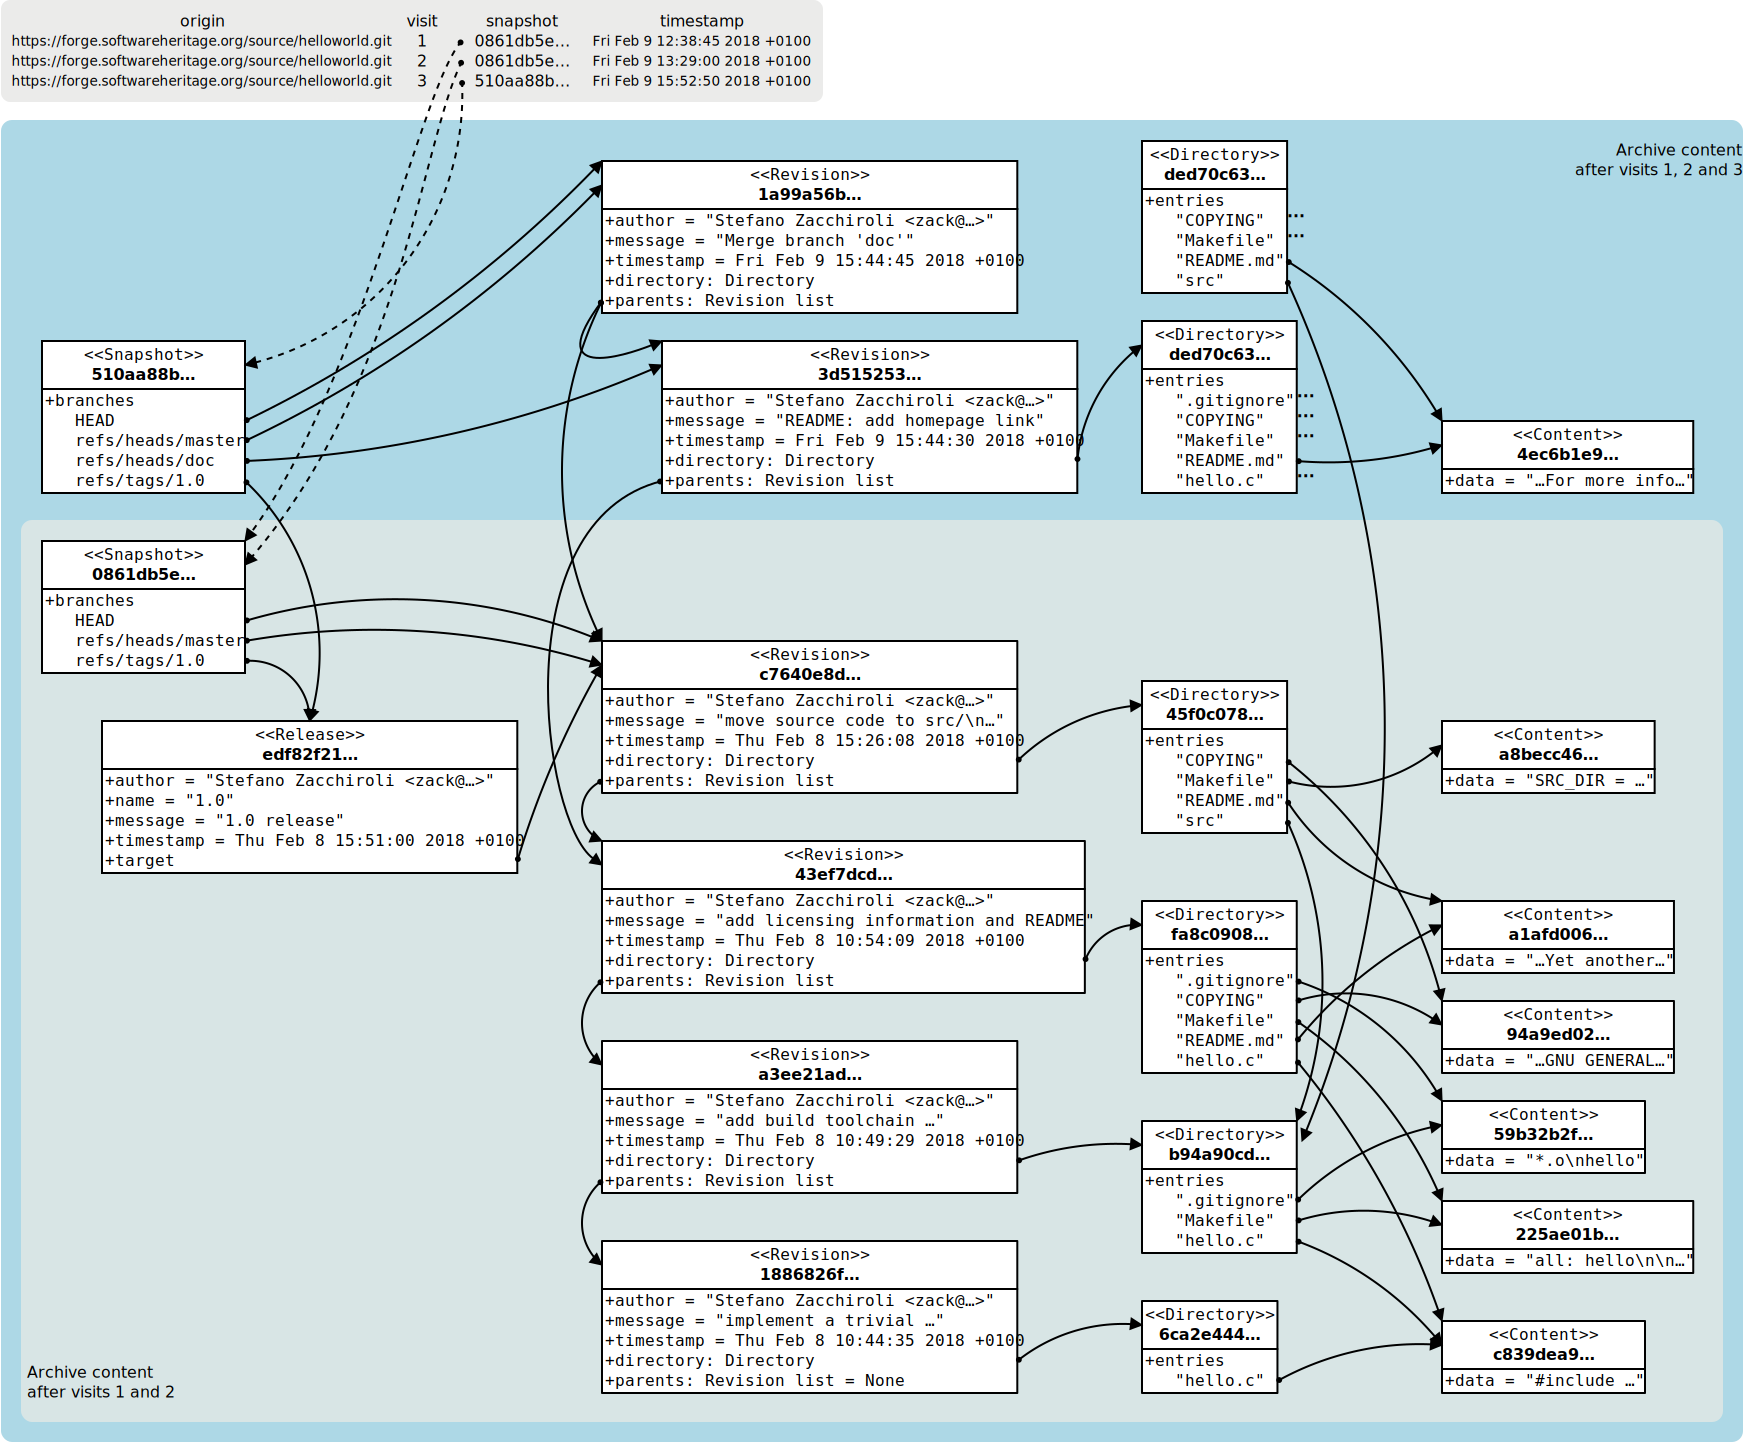
\includegraphics[height=7.5cm]{../img/swh-merkle-dag}
    %     \end{figure}
    % \end{frame}

    % \begin{frame}
    %     \frametitle{Graph statistics}
    %     \begin{columns}
    %         \column{.50\textwidth}
    %         \begin{block}{Graph topology}
    %             \begin{itemize}
    %                 \item $\approx$ 20 billion nodes
    %                 \item $\approx$ 220 billion edges
    %             \end{itemize}
    %         \end{block}

    %         \column{.50\textwidth}
    %         \begin{block}{Software artifacts}
    %             \begin{itemize}
    %                 \item $\approx$ 150 million software projects
    %                 \item $\approx$ 2 billion commits
    %                 \item $\approx$ 10 billion source code files
    %             \end{itemize}
    %         \end{block}
    %     \end{columns}
    % \end{frame}

    % vcs
    % archive

    \section{Making Software Data Available for Mining}

    \begin{frame}
        \frametitle{Requirement analysis for Empirical Software Engineering}

        \pdfpcnote{%
            The first thing we need is to understand the kinds of studies that
            researchers might want to perform on this data. To get a better
            understanding of that, I reviewed 54 papers from the MSR conference
            and categorized the different types of data that researchers
            usually make use of in their studies.
            \\\\
            A lot of these use cases require being able to efficiently query
            the graph of software development...
        }

        \begin{block}{Identifying researchers need}
            Literature review of \textbf{54 papers} from the Mining Software
            Repositories conference (MSR~2019).
        \end{block}

        \begin{block}{Categories of requested data}
            \begin{itemize}
                \item Blobs
                \item Filesystem hierarchy (\emph{file names, directories})
                \item History graph (\emph{revisions})
                \item Content search (\emph{full-text search index})
                \item Provenance (\emph{backwards index})
                \item Commit diffs
                \item Community graph (\emph{revision authors})
                \item Dependency data
            \end{itemize}
        \end{block}
    \end{frame}

    \begin{frame}
        \frametitle{Data volume challenges}
        \pdfpcnote{%
            But the thing is that this volume of data is completely
            unmanageable for most researchers. It doesn't fit on a single
            machine and so it often requires distributed approaches. Just
            downloading it takes entire months.\\
            Also, its structure makes it hard to analyze because of the high
            deduplication, which makes it a very entangled structure where
            parallel approaches are not necessarily straightforward.
            \\\\
            So in my thesis in present three different approaches to reduce the
            amount of data that researchers need to have **locally**.
            \\\\
            The first one is sampling, giving ways to access a small limited
            set of data.
            The second one is to help them query the graph remotely by putting
            the graph on cloud-based distributed computing platforms.
            The last one is to compress the data so that it can actually fit on
            a single machine to be analyzed locally.
        }

        \begin{block}{Local analysis}
            Handling data at that scale is a hard practical problem for
            researchers:
            \begin{itemize}
                \item Data does not fit on a single machine
                \item Downloading this volume of data can take months
                \item High deduplication: entangled structure, hard to
                    parallelize
            \end{itemize}
        \end{block}

        \begin{block}{Approaches addressed in this thesis}
            \begin{itemize}
                \item Sampling: access limited amounts of data
                \item Scale-out: platform for distributed computing
                \item Scale-up: compression
            \end{itemize}
        \end{block}
    \end{frame}

    \begin{frame}
        \frametitle{The Vault}

        \pdfpcnote{%
            The first thing you could do to analyze many repositories at once
            is to just download them one by one. In the archive there's no
            longer a notion of "repository" because everything is deduplicated.
            So I propose a new tool called the Vault to reconstitute these
            repositories by computing the transitive closure of a given
            artifact.
            \\\\
            We were able to use this for a few mining experiments that required
            up to tens of thousands of repositories at once. It's really
            convenient in that it doesn't require any kind of special analysis
            tool, because in effect you're just downloading the repository
            itself and you can study it like you study any repository. However,
            you lose all the deduplication, so you no longer have this map of
            relationships between software objects.
        }

        \begin{block}{}
            The \textbf{Vault}: Download single directories or entire
            repositories.
        \end{block}

        \begin{center}
            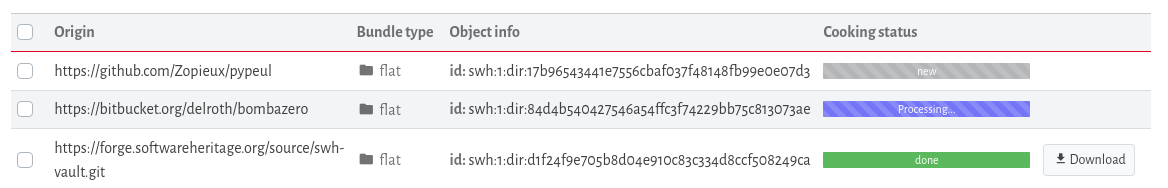
\includegraphics[width=\linewidth]{img/vault.png}
        \end{center}

        \begin{block}{}
            \begin{itemize}
                \item Retrieves the transitive closure of a
                    given object and bundles it in a tarball.
                \item Serves as a cache for downloadable tarballs.
                \item Scales up to tens of thousands of repositories
            \end{itemize}
        \end{block}

        \begin{block}{}
            \begin{itemize}
                \item \textbf{Pro}: does not require any special analysis tool
                \item \textbf{Con}: no deduplication (larger size, loss of
                    information)
            \end{itemize}
        \end{block}
    \end{frame}

    \begin{frame}[fragile]
        \frametitle{SwhFS}

        \pdfpcnote{%
            Another option we propose for sampling is the Software Heritage
            Filesystem, a way to expose the contents of the archive as a
            virtual filesystem. It works by lazily fetching the files and
            directories from the archive when the user accesses them.
            \\\\
            Like for the Vault, this is really useful for small-scale
            experiments because it doesn't require any specialized tools, but
            it's not suitable for exhaustive analyses of the graph.
            As an example, here is a simple way to count the number of lines of
            Javascript code in a given revision.
            \\\\
            So the Vault and this filesystem are the two ways we make small
            sets of data easily accessible for software mining. But our main
            goal is universal software mining, we want to be able to run more
            exhaustive experiments...
        }

        \begin{block}{}
            The \textbf{Software Heritage Filesystem}: a virtual FUSE
            filesystem to mount the archive as a local directory.

            \begin{itemize}
                \item Useful for prototyping
                \item Easy to exploit with common CLI tools \\
                    → Local file hierarchy maps well with archived repositories
                \item Suited for small-scale experiments
            \end{itemize}

            \footnotesize
            \begin{thebibliography}{swhfs}
                \bibitem{swhfs2020} Thibault Allançon, Antoine Pietri, Stefano Zacchiroli\newblock
                The Software Heritage Filesystem (SwhFS): Integrating Source Code Archival with Development\newblock
                ICSE 2021, IEEE\newblock
            \end{thebibliography}
        \end{block}

        \begin{block}{}
            \begin{minted}{console}
$ swh fs mount swhfs/
$ cd swhfs/archive/swh:1:rev:9d76c0b163675505d1a901e5fe5249a2c55609bc
$ find root/src/ -type f -name ’*.js’ | xargs cat | wc -l
10136
            \end{minted}
%             \begin{minted}{console}
% $ cd archive/swh:1:dir:1fee702c7e6d14395bbf5ac3598e73bcbf97b030
% $ grep -i antenna THE_LUNAR_LANDING.s | cut -f 5
% # IS THE LR ANTENNA IN POSITION 1 YET
% # BRANCH IF ANTENNA ALREADY IN POSITION 1
%             \end{minted}
        \end{block}
    \end{frame}

    \begin{frame}
        \frametitle{The Software Heritage Graph Dataset}

        \pdfpcnote{%
            So we present the Software Heritage Graph dataset, which is an
            export of the entire graph of software development, without the
            file contents -- just the graph.
            \\\\
            We provide it in two different formats, a set of relational tables
            in columnar format that can be used in classic distributed
            computing platforms like Spark or Hadoop, and one that is more
            graph oriented, a set of edges that you can import in graph
            processing platforms like Neo4J or Amazon Neptune.
            \\\\
            Of course you can just download this dataset and process them on
            your own infrastructure, but the main idea here is to reduce
            frictions and costs, so we have these available as public datasets
            on Amazon Athena and Azure Databricks, that anyone can just query
            without having to pay for the storage.
            \\\\
            Let's see a few examples of experiments that this allows us to
            perform.
        }

        \begin{block}{}
            The \textbf{Software Heritage Graph Dataset}: a snapshot of the
            entire graph of software development (without the file contents).

            \footnotesize
            \begin{thebibliography}{msr2019}
                \bibitem{swhgraph2019} Antoine Pietri, Diomidis Spinellis, Stefano Zacchiroli\newblock
                The Software Heritage graph dataset: public software development under one roof\newblock
                Mining Software Repositories 2019\newblock
            \end{thebibliography}
        \end{block}

        \begin{block}{Formats}
            \begin{itemize}
                \item A set of \emph{relational tables} in columnar format for
                    scale-out processing
                \item A \emph{graph edges} format for use in graph databases
                    and graph analysis platforms
            \end{itemize}
        \end{block}

        \begin{block}{Availability}
            \begin{itemize}
                \item Downloadable for local use
                \item Cloud processing platforms: Amazon Athena, Azure
                    Databricks
            \end{itemize}
        \end{block}
    \end{frame}

    \begin{frame}[fragile]{Example queries}
        \pdfpcnote{%
            This query is to find the most common "actions" that developers
            perform in their commits, which are generally the first words of
            the commit message. So using Amazon Athena, in just a few lines of
            SQL we are able to extract this information from 1.1 billion
            revisions, and in just 30 seconds we get this result, with "update"
            being the most common action followed by "merge".
        }

        \begin{block}{Most frequent first commit words}
            \begin{minted}[fontsize=\small]{sql}
SELECT COUNT(*) AS c, word FROM (
  SELECT LOWER(REGEXP_EXTRACT(FROM_UTF8(
  message), 'ˆ\w+')) AS word FROM revision)
WHERE word != ''
GROUP BY word ORDER BY COUNT(*) DESC LIMIT 5;
            \end{minted}

            \begin{center}
                \begin{tabular}{rl}
                    Count & Word\\
                    \hline
                    \num{71338310} & update\\
                    \num{64980346} & merge\\
                    \num{56854372} & add\\
                    \num{44971954} & added\\
                    \num{33222056} & fix\\
                \end{tabular}
            \end{center}
        \end{block}

        \begin{block}{}
            Analyzes 1.1 billion revision messages in 30 seconds.
        \end{block}
    \end{frame}

    \begin{frame}[fragile]{Example queries}
        \pdfpcnote{%
            For a more complex query, here we're trying to answer the question
            of whether there's been a change in the proportion of commits
            made during the week-end. Maybe our hypothesis is that people are
            changing their work/life balance, something like that. And again we
            can analyze all the commits in the dataset in just a few seconds,
            and we get these results. The trend appears stable over time, with
            a flat best fit line, so there is no sign of such a shift.
        }

        \begin{columns}
            \column{0.5\textwidth}
            \begin{block}{Weekend work}
                \inputminted[fontsize=\tiny, firstline=3]{sql}{../codesamples/graph-dataset/weekend-work.sql}
            \end{block}
            \column{0.5\textwidth}
            \begin{center}
                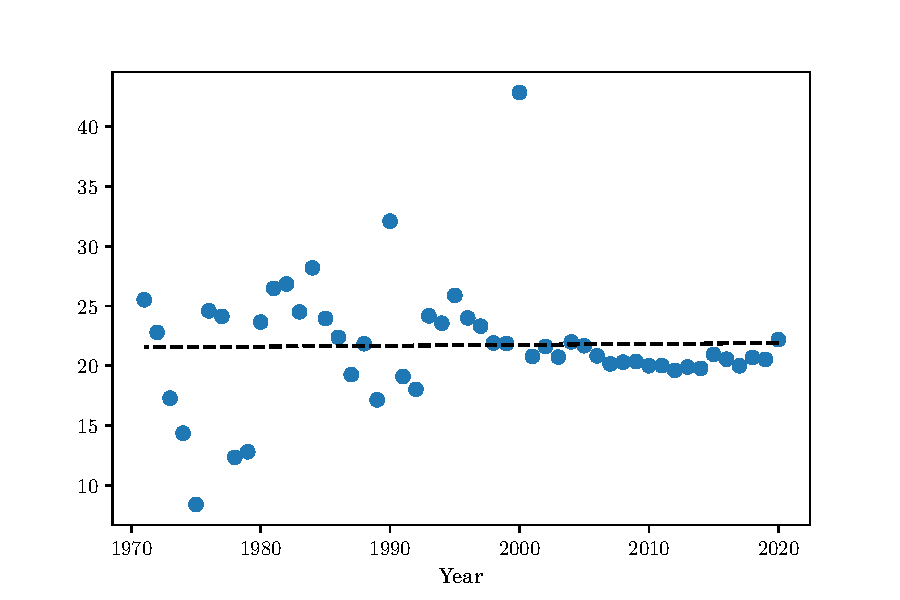
\includegraphics[width=\linewidth]{../img/graph-dataset/weekend-work}
            \end{center}
        \end{columns}

        \begin{block}{}
            Analyzes 1.1 billion revision timestamps in 7 seconds.
        \end{block}
    \end{frame}

    \begin{frame}
        \frametitle{Recursive queries}
        \pdfpcnote{%
            So this scale-out approach of massively distributing computations
            on extremely large volumes of data works really well for
            embarrassingly parallel queries, that can be just trivially
            distributed on clusters of machine.
            \\\\
            But for a lot of research use cases, we need to exploit the
            recursive structure of the graph, run actual graph algorithms on
            this dataset like getting transitive closures or computing
            connected components. And doing this on scale-out solutions is
            completely cost prohibitive, we tried that on Spark using the
            GraphFrames library and it required spawning a cluster of 80 nodes
            for 4 hours, which costs approximately 5000 dollars.
            \\\\
            So now the question is, could we make it accessible to researchers
            to run complex graph algorithms on the dataset of software
            development?
        }
        \begin{block}{}
            \begin{itemize}
                \item This approach works really well for
                    \textbf{embarrassingly parallel} queries
                \item Scale-out solutions are less efficient for
                    \textbf{recursive queries} that exploit the
                    hierarchical/structured nature of the graph
                \item BFS Traversal of the graph on Spark: 4 hours, 80
                    nodes (!), 5000 USD
            \end{itemize}
        \end{block}

        \begin{block}{Research question}
            Can recursive graph algorithms be performed in an
            accessible and cost-efficient way?
        \end{block}
    \end{frame}

    % \begin{frame}[fragile]{Example queries}
    %     \begin{block}{Spark: Connected components size distribution}
    %         \inputminted[fontsize=\small]{sql}{../codesamples/graph-dataset/spark-cc.py}
    %     \end{block}

    %     \begin{block}{}
    %         \textbf{Warning}: distributed graph algorithms on Spark are very
    %         expensive (\textasciitilde{}5000 USD for the entire graph with
    %         Azure Databricks).
    %     \end{block}
    % \end{frame}

    \section{Graph Compression}

    \begin{frame}
        \frametitle{Compression approach}

        \pdfpcnote{%
            The idea here is to compress the graph of software development in a
            way that makes it possible to analyze it on a single machine.
            One major advantage of this approach is that wouldn't need to write
            distributed versions of the graph algorithms, which can often
            require a lot of research in itself, and makes it less
            accessible.\\
            If done efficiently, we expect it to be a lot cheaper
            than distributed approaches, so that should allow us to run
            exhaustive analyses very quickly and gain a better understanding of
            the graph.
            \\\\
            We're not proposing new graph compression techniques here, but
            importing and evaluating existing ones for our specific domain. In
            particular we're going to look at techniques used to compress the
            graph of the Web, and see if they can be adapted for the graph of
            software development.
        }

        \begin{block}{}
            \textbf{Objective}: Analyzing the \emph{entire graph of public
            software development} on a single machine.

            \footnotesize
            \begin{thebibliography}{swhgraphcomp}
                \bibitem{Boldi2020} Paolo Boldi, Antoine Pietri, Sebastiano Vigna, Stefano Zacchiroli
                \newblock Ultra-Large-Scale Repository Analysis via Graph Compression
                \newblock SANER 2020, 27th Intl. Conf. on Software Analysis, Evolution and Reengineering. IEEE
            \end{thebibliography}
        \end{block}

        \begin{block}{Advantages}
            \begin{itemize}
                \item Simpler for prototyping, no need to write distributed
                    algorithms
                \item Cheaper than scale-out processing
                \item Allows us to run exhaustive analyses quickly
            \end{itemize}
        \end{block}

        \begin{block}{Compression techniques}
            Existing compression algorithms used with the
            \textbf{graph of the Web}.
        \end{block}
    \end{frame}

    \begin{frame}{Compression pipeline}
        \pdfpcnote{%
            The graph of the web has a good property for compression, which is
            that when you order all its nodes lexicographically by URL, you get
            an order that preserves locality of the nodes in the graph. Similar
            URLs will be in the same neighborhood of nodes.
            And having this node locality is a key property to be able to
            compress adjacency lists efficiently.
            \\\\
            For the graph of software development we don't have that property,
            because the node identifiers are just randomly distributed
            cryptographic hashes. However we can reconstitute a node order that
            has this locality information by doing a breadth-first traversal.
            \\\\
            The idea of this pipeline is that we will first compress the graph
            using a random node ordering, which will give us a really bad
            compression ratio. But starting from that graph, we can run a
            BFS and use that new node ordering to recompress the graph and
            achieve a better compression ratio.
        }

        \begin{block}{Web graph → Software development graph: (re)establishing locality}
            Key for good compression of adjacency lists is a \alert{node
            ordering} that ensures \textbf{neighbor locality}.
            \begin{itemize}
                \item Lexicographically-ordered URLs in the Graph of the Web
                    have this property.
                \item It is \emph{not} the case with cryptographic Merkle
                    IDs\ldots{}
                \item \ldots but is the case \emph{again} after a
                    breadth-first traversal
            \end{itemize}
        \end{block}
        \vspace{-0.7cm}
        \begin{center}
            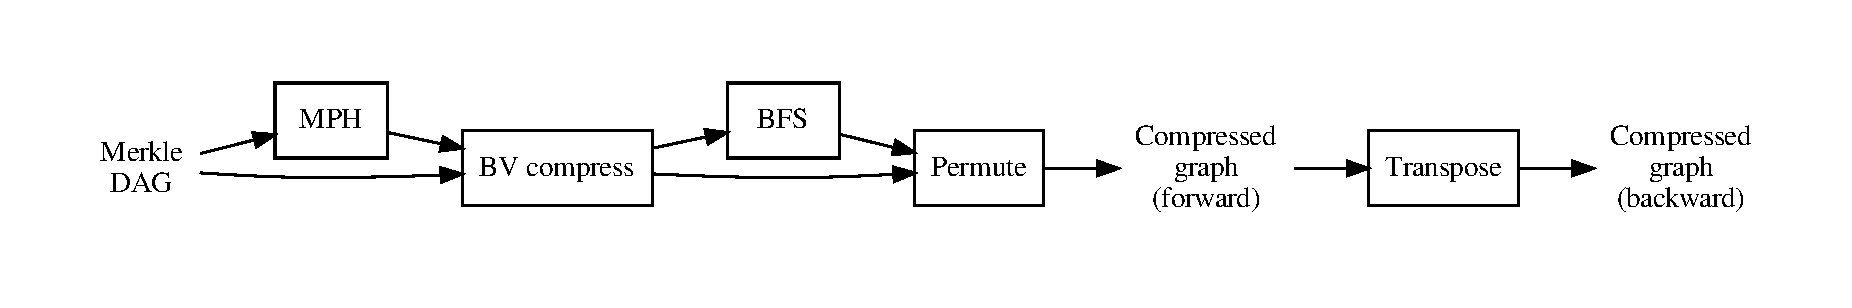
\includegraphics[width=1\linewidth]{../img/compression/compression_steps-nofiles}
        \end{center}
        \vspace{-1cm}
        \begin{itemize}
            \item \alert{MPH:} minimal perfect hash, mapping Merkle IDs to 0..N-1 integers
            \item \alert{BV compress:} Boldi-Vigna compression (based on MPH order)
            \item \alert{BFS:} breadth-first visit to renumber
            \item \alert{Permute:} update BV compression according to BFS order
        \end{itemize}
    \end{frame}

    \begin{frame}{Compression results}
        \pdfpcnote{%
            We ran this compression pipeline on the graph dataset using the
            WebGraph framework, on a server with 24 CPUs and 750 GB of RAM.
            The compression only takes 6 days, and from the 6 TB input we
            obtain a compressed graph of only 91 GB. We can also produce a
            transposed graph for backward traversals, and this one is 83 GB.
            Those figures only include the graph structure of nodes and edges,
            but not the data associated with them (like file contents or commit
            messages...)
            \\\\
            Now it's definitely possible to put these graphs in RAM, at least
            on a high-end machine. We ran a benchmark to see how fast it was to
            run algorithms on the entire graph, and a full traversal takes less
            than 2 hours.
        }
        \begin{block}{}
            We ran the compression pipeline on the input corpus using the
            \textbf{WebGraph} framework (Boldi, Vigna 2004).
            % \begin{thebibliography}{}
            %     \footnotesize
            %     \bibitem{BoVWFI} Paolo Boldi and Sebastiano Vigna.
            %     \newblock The WebGraph framework I: Compression techniques
            %     \newblock WWW 2004: 13th Intl. World Wide Web Conference. ACM
            % \end{thebibliography}
        \end{block}

        \begin{block}{}
            \begin{itemize}
                \item Server equipped with 24 CPUs and 750 GB of RAM
                \item \textbf{Compression time}: 138 hours (6 days)
                \item \textbf{Compression efficiency}: 6 TiB edge file → 91 GiB
                    forward, 83 GiB transposed
            \end{itemize}
        \end{block}

        \begin{block}{Benchmark}
            Full traversal: 1h48min (1.81 M nodes/s) on a single thread\\
            ⇒ Huge improvement over Spark (4 h, 80 nodes, 5000 USD)
        \end{block}

    \end{frame}

    \begin{frame}{LLP compression}
        \pdfpcnote{%
            It's possible to push the compression even further with Layered
            Label Propagation, which is another algorithm that can discover
            locality information between nodes.
            The way it works is by assigning random labels to node and
            propagating them to they neighbors, which generates clusters of
            nodes all located in the same neighborhood.
            \\\\
            This step goes after the BFS in the pipeline, so we get better and
            better compression at every step.
            It has a big tradeoff in that it requires a lot more runtime
            memory, which is not always achievable depending on your hardware
            configuration, but the compression ratio we obtain is really
            impressive, it reduces the size of the graph 35\% further.
        }
        \begin{block}{}
            \textbf{Layered Label Propagation}: algorithm to uncover better
            locality-preserving node orderings (Boldi et al. 2010)
            % \begin{thebibliography}{Foo Bar, 1969}
            %     \small \vspace{-2mm}
            %     \bibitem{Boldi2010} Paolo Boldi, Marco Rosa, Massimo Santini, Sebastiano Vigna
            %     \newblock Layered Label Propagation: A MultiResolution Coordinate-Free Ordering for Compressing Social Networks
            %     \newblock WWW 2010: 20th Intl. World Wide Web Conference. ACM
            % \end{thebibliography}
        \end{block}
        \begin{block}{}
            \begin{itemize}
                \item Algorithm to uncover locality information
                \item Propagates labels on random nodes to discover neighborhoods
                \item Even more impressive compression ratio (91 GiB → 60 GiB,
                    reduced by \textasciitilde{}35\%)
                \item Compression requires more runtime memory
            \end{itemize}
        \end{block}
    \end{frame}

    \begin{frame}{Graph Attributes}
        \pdfpcnote{%
            Up until now we have only compressed the structure of the graph but
            not the attributes stored on the nodes and the edges, like commit
            messages, timestamps, etc. But this data is needed for a lot of use
            cases, like if you want to find the earliest commit in which a
            unique file has ever been found.
            \\\\
            In my thesis, I propose various designs to actually store this data
            so that it can be accessed during graph traversals. These
            techniques exploit the fact that node IDs are contiguous to store
            them as binary arrays on disk. We can mmap these arrays at runtime
            depending on which kinds of data we need access to.
            \\\\
            Storing data on edges is a bit more involved, but there is built in
            support in WebGraph to achieve that. I use other techniques to
            compress the attributes on the edges, like a MPH on the file names
            to only have to store them once.
        }
        \begin{block}{Node attributes}
            \begin{itemize}
                \item The compressed in-memory graph structure has \alert{no attributes}
                \item Usual data design is to exploit the 0..N-1 integer ranges to \alert{memory map
                    \emph{node} attributes} from secondary storage (node ID →
                    node attribute)
                    \begin{itemize}
                        \item We do this for node types (mapping: 4 GiB),
                            timestamps (mapping: 149 GiB), etc.
                        \item Data structures: integer/byte arrays, front-coded
                            string lists, etc.
                    \end{itemize}
            \end{itemize}
        \end{block}
        \begin{block}{Edge attributes}
            \begin{itemize}
                \item Built-in WebGraph support for attributes on the
                    \alert{edges} (generally integers)
                \item We convert \emph{file names} to integers using a MPH
            \end{itemize}
        \end{block}
        % \begin{block}{Disk/memory consideration}
        %     \begin{itemize}
        %         \item Labels and mappings can be either in RAM or
        %             \texttt{mmap()}-ed from disk
        %         \item Time/memory tradeoff, depends on access patterns, intensive
        %             workloads etc.
        %     \end{itemize}
        % \end{block}
    \end{frame}

    \begin{frame}[fragile]{Graph Querying}
        \pdfpcnote{%
            Once we have this compressed graph, we need to make it actually
            accessible for researchers who want to run experiments on it. We
            have a very basic API to write graph algorithms, but it only
            provides very low level primitives like the successors() function
            to get the adjacency list of a node. A big issue here is that this
            requires local access to the server, so you can't really set it up
            as a service that researchers can query.
            \\
            If we want to do better we need to build a traversal language on
            top of this.
        }
        \begin{block}{}
            \textbf{Option 1}: Write a traversal algorithm using Java
            graph primitives
        \end{block}
        \begin{minted}[fontsize=\scriptsize,highlightlines={8}]{java}
HashSet<Long> visited = new HashSet<>();
Stack<Long> stack = new Stack<>();
stack.push(srcNodeId);
visited.add(srcNodeId);

while (!stack.isEmpty()) {
    long currentNodeId = stack.pop();
    LazyLongIterator it = graph.successors(currentNodeId);
    for (long neighborNodeId; (neighborNodeId = it.nextLong()) != -1; ) {
        if (!visited.contains(neighborNodeId)) {
            stack.push(neighborNodeId);
            visited.add(neighborNodeId);
        }
    }
}
        \end{minted}
        \begin{block}{}
            \begin{itemize}
                \item Efficient but low-level \& requires local access to the
                    graph server.
                \item Simpler/remote querying ⇒ need to build traversal query
                    language
            \end{itemize}
        \end{block}
    \end{frame}

    \begin{frame}[fragile]
        \frametitle{Graph Querying}
        \pdfpcnote{%
            So we built a simple HTTP API which can be used to run simple
            traversals remotely. It has a few base primitives, like getting the
            neighbors or the leaves of a node, or return its entire transitive
            closure. It can't do more complex queries like traversals starting
            from multiple nodes at the same time, but it does have a few
            options like a way to add constraints on the types of edges
            traversed by the algorithm.
            \\\\
            Now that we have built this framework to cheaply run exhaustive
            experiments on the compressed graph, we can use it to try to
            understand the structure of this giant graph of software
            development.
        }

        \begin{block}{}
            \textbf{Option 2}: HTTP API for simple graph traversals

            \begin{itemize}
                \item Generic remote API for graph traversals, Java/Python/aiohttp backend
                \item Limited to simple DFS from a single node (forward or
                    backward graph)
                \item Traversal types: neighbors, leaves, all nodes, all edges
                \item Supports edge-type filtering
            \end{itemize}
        \end{block}

        \begin{minted}[fontsize=\scriptsize]{text}
> GET /leaves/swh:1:rev:f39d[...]2a35?direction=backward
swh:1:ori:634a2b699d442aa9abd5008f379847816f54ab85
swh:1:ori:571a86b198c6c66ef33025249f7e455b529aae65
swh:1:ori:c15194d6cb59a6d32777ca3b287ea6664d540df3
...

> GET /visit/nodes/swh:1:rev:c6df[...]fc28?edges=rel:rev,rev:rev
swh:1:rel:c6df0a7ef73ca90825f1472b8a3c5f7a2ce3fc28
swh:1:rev:c8448ff2f9234332f0bc25dc3a13031f8ab3c73c
swh:1:rev:4b63dbd4e782e74bdc050c4579381d29b4bd41c0
...
        \end{minted}
    \end{frame}

    % \begin{frame}
    %     \frametitle{Graph Subdatasets}

    %     \begin{block}{Generating representative subgraphs}
    %         \begin{itemize}
    %             \item Useful for smaller-scale experimentation, prototyping
    %             \item Focusing analysis on a relevant subset
    %             \item Representative samples → transitive closure of a subset
    %                 of origins
    %             \item Use a fitted log model to estimate the size of the
    %                 resulting subgraph
    %         \end{itemize}
    %     \end{block}

    %     \begin{center}
    %         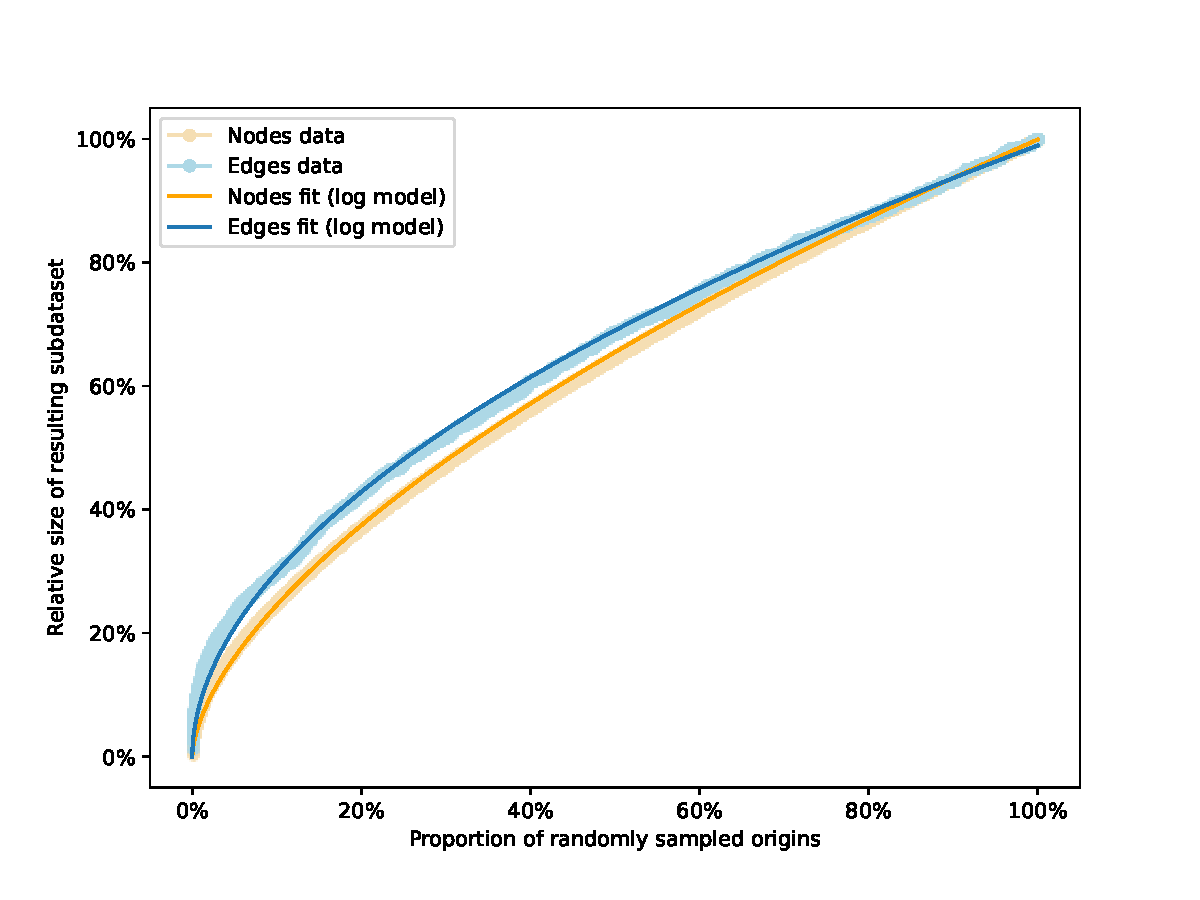
\includegraphics[width=.5\linewidth]{../img/graph-exploitation/subdataset_size_function_fit.pdf}
    %     \end{center}
    % \end{frame}

    \section{Graph Topology of Software Development}

    \begin{frame}
        \frametitle{Graph Topology: Research Questions}
        \pdfpcnote{%
            As we said before, the graph dataset is a very meaningful object
            for software mining researchers, because it materializes all the
            relationships between all the software objects available publicly.
            This creates a very complex structure that has never been
            empirically studied before, but the now the compressed graph
            framework can be used to run exhaustive studies on it.
            \\\\
            So the first thing we want to do is to compute the key metrics that
            characterize complex networks in general, like degree
            distributions, connected components, distances between roots and
            leaves and clustering coefficient. I computed all these metrics on
            the entire graph but also on its different layers, so now I can
            show you what they actually tell us about the graph. And from there
            we can deduce potential implications for software mining, like ways
            to distribute computations on the graph efficiently, and
            methodological implications for empirical studies.
        }

        \begin{block}{}
            The Software Heritage Graph Dataset materializes a \emph{network of
            relationships between software artifacts} which has not yet been
            empirically studied as a whole.
        \end{block}

        \begin{block}{Research questions}

            \begin{itemize}
                \item What is the network topology of the graph of software
                    development?

                    Network topology metrics: Degree distributions, connected
                    components, distance between roots and leaves, clustering
                    coefficient.

                \item What do these metrics tell us about this graph and its
                    layers?
                    \begin{itemize}
                \item Best approaches for large scale analysis?
                \item Methodological implications for software mining?
                    \end{itemize}
            \end{itemize}

            The \textbf{compressed graph framework} allows us to answer these
            questions experimentally.

            \footnotesize
            \begin{thebibliography}{swhforks}
                \bibitem{swhforks} Antoine Pietri, Guillaume Rousseau, Stefano Zacchiroli\newblock
                Determining the intrinsic structure of public software development history\newblock
                Mining Software Repositories 2020\newblock
            \end{thebibliography}
        \end{block}
    \end{frame}

    % \begin{frame}
    %     \frametitle{Graph layers}

    %     \begin{block}{}
    %         We study the topology of the graph as a whole, but also of its
    %         different semantic layers:
    %     \end{block}

    %     \begin{center}
    %         \scalebox{0.6}{\begin{tikzpicture}[scale=0.8, label distance=1pt]
	\begin{pgfonlayer}{nodelayer}
		\node [draw, shape=ellipse, style=originfill] (origin) at (2, 2) {Origin};
		\node [draw, shape=ellipse, style=snapshotfill] (snapshot) at (2, 0) {Snapshot};
		\node [draw, shape=ellipse, style=releasefill] (release) at (2, -2) {Release};
		\node [draw, shape=ellipse, style=revisionfill] (revision) at (2, -4) {Revision};
		\node [draw, shape=ellipse, style=directoryfill] (directory) at (2, -6) {Directory};
		\node [draw, shape=ellipse, style=contentfill] (content) at (2, -8) {Blob};
		\node [style=none] (1) at (-1.25, -5.25) {};
		\node [style=none] (2) at (4, -5.25) {};
		\node [style=none] (3) at (-1.25, -8.75) {};
		\node [style=none] (4) at (4, -8.75) {};
		\node [style=none] (5) at (-1.25, 2.75) {};
		\node [style=none] (6) at (4, 2.75) {};
		\node [style=none] (7) at (-1.25, -0.75) {};
		\node [style=none] (8) at (4, -0.75) {};
		\node [style=none] (9) at (-1, -3.25) {};
		\node [style=none] (10) at (-1, -4.75) {};
		\node [style=none] (11) at (4, -4.75) {};
		\node [style=none] (12) at (4, -3.25) {};
		\node [style=none] (13) at (-1.25, -1) {};
		\node [style=none] (14) at (7, -1) {};
		\node [style=none] (15) at (-1.25, -5) {};
		\node [style=none] (16) at (7, -5) {};
		\node [style=none] (17) at (-1.5, 3) {};
		\node [style=none] (18) at (-1.5, -9) {};
		\node [style=none] (19) at (10, -9) {};
		\node [style=none] (20) at (10, 3) {};
	\end{pgfonlayer}
	\begin{pgfonlayer}{edgelayer}
		\draw [style=cluster] (5.center) to (6.center);
		\draw [style=cluster] (6.center) to (8.center);
		\draw [style=cluster] (8.center) to (7.center);
		\draw [style=cluster] (5.center) to (7.center);
		\draw [style=cluster] (13.center) to (14.center);
		\draw [style=cluster] (14.center) to (16.center);
		\draw [style=cluster] (16.center) to (15.center);
		\draw [style=cluster] (15.center) to (13.center);
		\draw [style=cluster] (9.center) to (10.center);
		\draw [style=cluster] (10.center) to (11.center);
		\draw [style=cluster] (11.center) to (12.center);
		\draw [style=cluster] (9.center) to (12.center);
		\draw [style=cluster] (1.center) to (3.center);
		\draw [style=cluster] (3.center) to (4.center);
		\draw [style=cluster] (1.center) to (2.center);
		\draw [style=cluster] (2.center) to (4.center);
		\draw [style=cluster] (17.center) to (18.center);
		\draw [style=cluster] (18.center) to (19.center);
		\draw [style=cluster] (19.center) to (20.center);
		\draw [style=cluster] (20.center) to (17.center);
		\draw [style=arrow] (origin) to (snapshot);
		\draw [style=arrow] (snapshot) to (release);
		\draw [style=arrow] (release) to (revision);
		\draw [style=arrow] (revision) to (directory);
		\draw [style=arrow] (directory) to (content);
		\draw [style=dashed arrow, draw=lightgray, bend right=60, looseness=0.75] (snapshot) to (content);
		\draw [style=dashed arrow, draw=lightgray, bend right=60, looseness=0.75] (snapshot) to (directory);
		\draw [style=dashed arrow, draw=lightgray, bend right=45] (release) to (directory);
		\draw [style=dashed arrow, draw=lightgray, bend right=45] (release) to (content);
		\draw [style=arrow, loop left, loop] (revision) to ();
		\draw [style=arrow, bend right] (directory) to (revision);
		\draw [style=arrow, loop left, loop] (directory) to ();
		\draw [style=arrow, bend right=60] (snapshot) to (revision);

        \draw [decorate, decoration={brace,raise=5pt,amplitude=10pt}] (6) to node [align=left, right=20pt, style=none] {Hosting\\ layer} (8);
        \draw [decorate, decoration={brace,raise=5pt,amplitude=5pt}] (12) to node [align=left, right=20pt, style=none] {Commit\\ layer} (11);
        \draw [decorate, decoration={brace,raise=5pt,amplitude=10pt}] (2) to node [align=left, right=20pt, style=none] {Filesystem\\ layer} (4);
        \draw [decorate, decoration={brace,raise=5pt,amplitude=10pt}] (14) to node [align=left, right=20pt, style=none] {History\\ layer} (16);
        \draw [decorate, decoration={brace,raise=5pt,amplitude=10pt}] (20) to node [align=left, right=20pt, style=none] {Full graph} (19);
	\end{pgfonlayer}
\end{tikzpicture}
}
    %     \end{center}
    % \end{frame}

    \begin{frame}
        \frametitle{Average degree}
        \pdfpcnote{%
            The first metric we can look at is the average degree of the graph,
            which is the average number of neighbors of all the nodes in the
            graph. We can compare this degree with other complex networks that
            have been studied in the literature, like social or collaboration
            networks.
            \\\\
            We can see that the graph is relatively sparse, with a degree of
            around 11. For comparison the social graph of Facebook has an
            average degree of 169. Another important thing is that this degree
            of 11 is largely dominated by the filesystem layer, which contains
            around 90\% of all the nodes in the graph. The commit layer is even
            more sparse, with an average degree of around one, which likely
            means it's mostly constituted of long chains.
        }
        \begin{block}{}
            Average number of neighbors of all the nodes in the graph

            % (e.g., social networks → number of friends/followers)
        \end{block}

        \begin{table}
            \centering
            \begin{tabular}[t]{l S[table-format=3.3]}
                \textbf{Dataset} & \textbf{Average degree} \\
                \hline
                % \textbf{swh-2020-history}    & 1.021 \\
                \textbf{swh-2020-commit}     & 1.022 \\
                % \textbf{swh-2020-hosting}    & 3.39 \\
                bitcoin-2013 & 6.4 \\
                dblp-2011 (Co-authorship)       & 6.8 \\
                \textbf{swh-2020}            & 11.0 \\
                \textbf{swh-2020-filesystem} & 12.1 \\
                twitter-2010      & 35.2 \\
                clueweb12                    & 43.1 \\
                uk-2014 (Web)               & 60.4 \\
                fb-2011 (Facebook)          & 169.0 \\
            \end{tabular}
        \end{table}
    \end{frame}

    \begin{frame}
        \frametitle{Out-degree distributions: filesystem layer}
        \pdfpcnote{%
            Here is the plot of the outdegree distribution of the filesystem
            layer, which corresponds to the distribution of the number of
            entries of each directory in the graph.
            \\\\
            This is how you read this frequency distribution: this shows that
            there are around 10^8 nodes with **exactly** 20 children. There's
            also a cumulative frequency distribution, in which you can see that
            there are around 10^9 nodes with **more** than 20 children.
            \\\\
            What we can see here is that there is not really a threshold
            effect after which the degrees are really unlikely, it decreases in
            something that looks like a power law. So there is not really a
            characteristic number of entries in a directory.
        }

        \begin{block}{}
            Distribution of the number of entries of each directory in the
            graph
        \end{block}

        \begin{figure}
            \centering
            \only<1,4>{%
                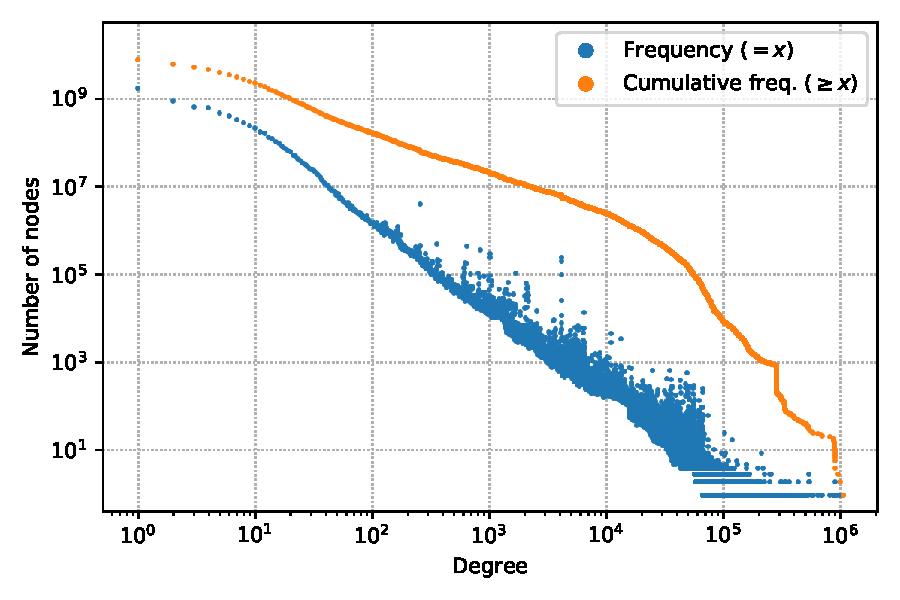
\includegraphics[width=0.5\linewidth]{img/topology/inout/dir+cnt_out}
            }
            \only<2>{%
                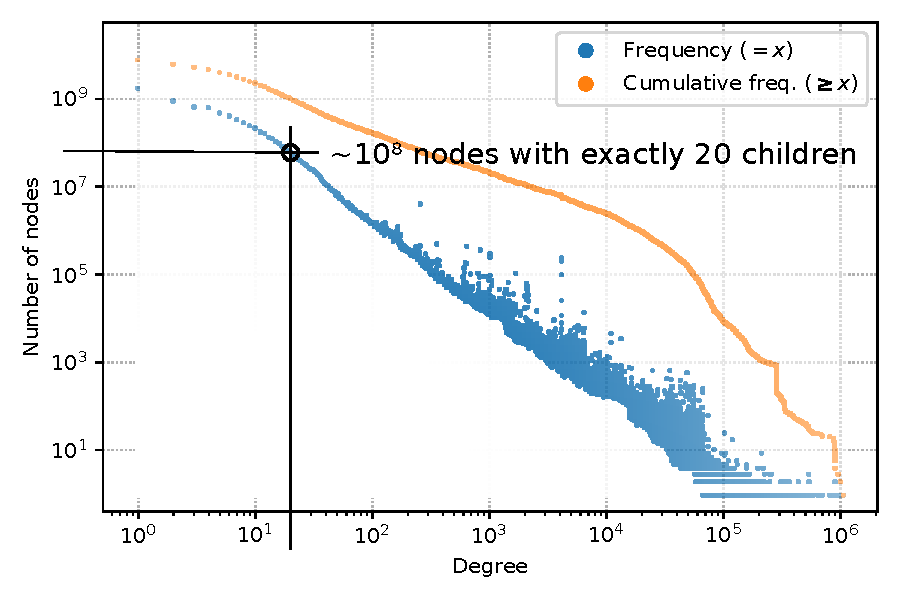
\includegraphics[width=0.5\linewidth]{img/topology/inout/dir+cnt_out_annotated}
            }
            \only<3>{%
                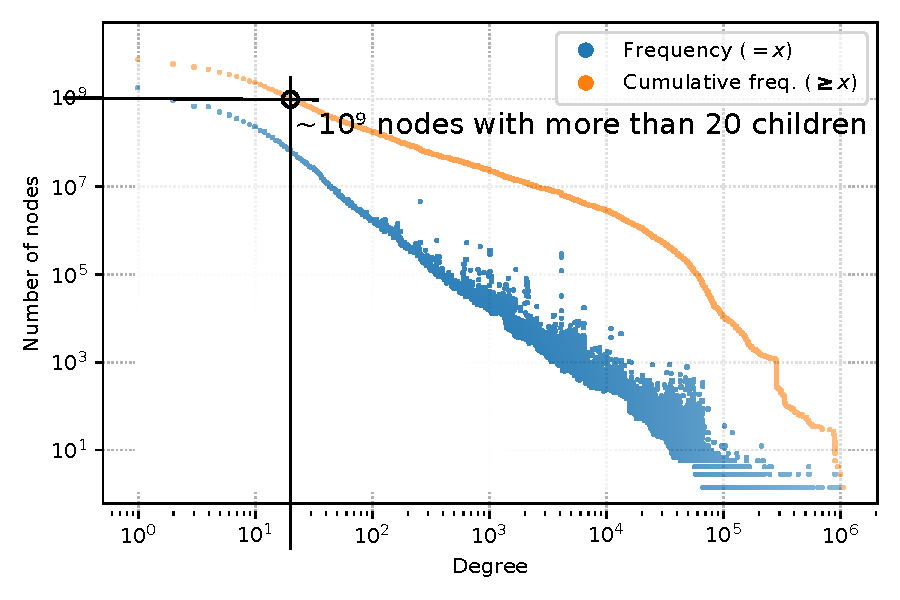
\includegraphics[width=0.5\linewidth]{img/topology/inout/dir+cnt_out_annotated_cum}
            }
        \end{figure}

        \begin{block}{}
            ⇒ No characteristic number of entries in a directory.
        \end{block}
    \end{frame}

    \begin{frame}
        \frametitle{Out-degree distributions: commit layer}
        \pdfpcnote{%
            It's very different in the commit layer. This shows the
            distribution of the number of parents of the commits in the graph.
            And here we can see a huge threshold effect, basically there are a
            lot of commits with only one parents, many commits with two
            parents, but after that it's mostly outliers. Keep in mind that
            this is a logarithmic scale, so there are three orders of magnitude
            between these two points.
            \\\\
            This happens because of development
            patterns, most commits will have only one parent, except for merge
            commits which generally have two. It's possible to make octopus
            merges with more than 3 parents, but it's exceedingly rare.
        }
        \begin{block}{}
            Distribution of the number of parents of each commit in the graph
        \end{block}

        \begin{figure}
            \centering
            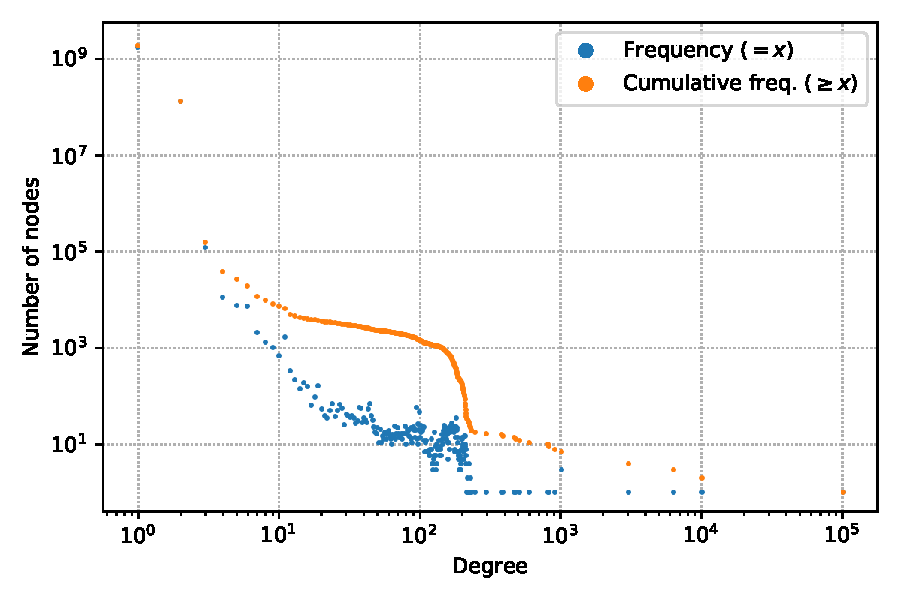
\includegraphics[width=0.5\linewidth]{img/topology/inout/rev_out}
        \end{figure}

        \begin{block}{}
            ⇒ Characteristic number of parents due to development patterns.
        \end{block}
    \end{frame}

    \begin{frame}
        \frametitle{Distance between roots and leaves}
        \pdfpcnote{%
            We can see a similar disparity in the distance between the roots
            and the leaves. For the filesystem layer, this corresponds to the
            depth of files in directory trees. Here there is a notable
            threshold effect: most of the files are less than 10-20 levels
            deep, and files deeper than that are very rare.
            \\\\
            Commit chains don't have characteristic lengths, they seem to
            decrease in what again looks like a power law, meaning their length
            is arbitrary.
        }

        \begin{figure}
            \begin{subfigure}{.49\textwidth}
                \centering
                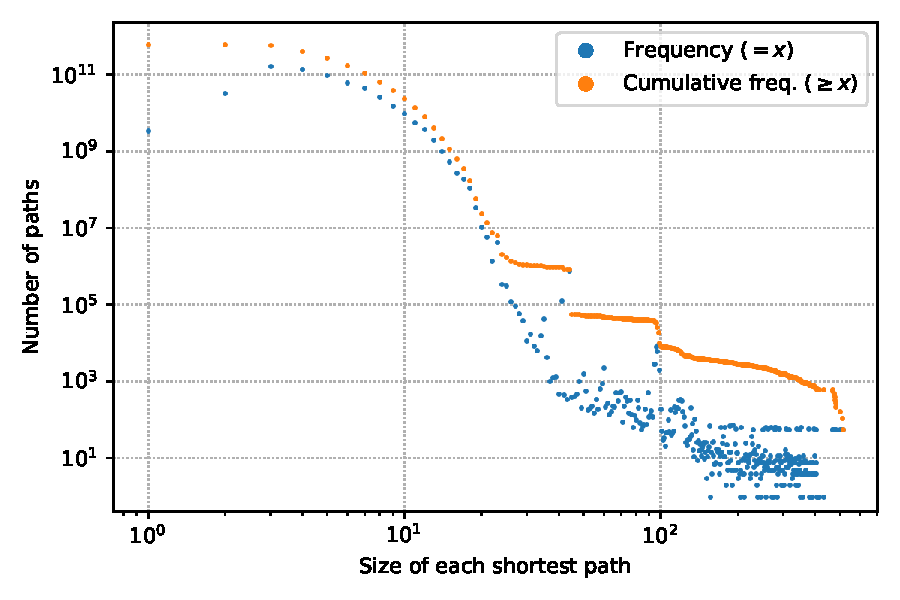
\includegraphics[width=\linewidth]{img/topology/shortestpath/dir+cnt}
                \caption{Depth of files in directory trees}
            \end{subfigure}\hfill
            \begin{subfigure}{.49\textwidth}
                \centering
                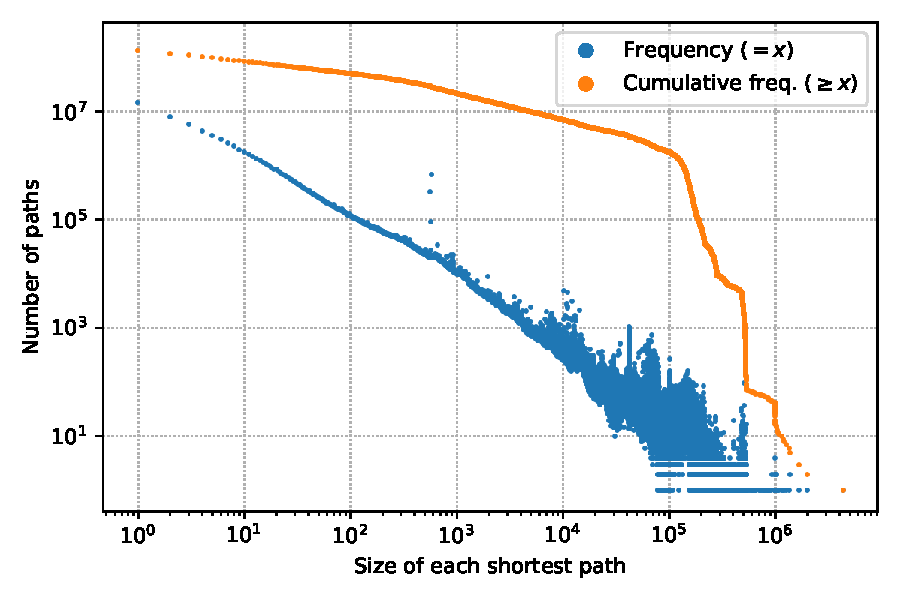
\includegraphics[width=\linewidth]{img/topology/shortestpath/rev}
                \caption{Length of commit chains}
            \end{subfigure}
        \end{figure}
    \end{frame}

    \begin{frame}
        \pdfpcnote{%
            An interesting metric is the size distribution of connected
            components. We use connected components to identify clusters of
            connected nodes but completely isolated from the
            rest of the graph. This is very useful, because if the graph is
            constituted a lot of small isolated island of software, it's really
            easy to shard the entire graph in distributed clusters. You can
            then just analyze each component separately without needing
            to synchronize the processes.
            \\\\
            Well, it turns out that this is not the case at all for the
            filesystem layer. more than 97\% of all the nodes are
            interconnected together in the giant component you see here. For
            the commit layer, this is a lot more doable, since the largest
            component only contains 3\% of the nodes.
        }
        \frametitle{Connected components}
        \begin{figure}
            \begin{subfigure}{.49\textwidth}
                \centering
                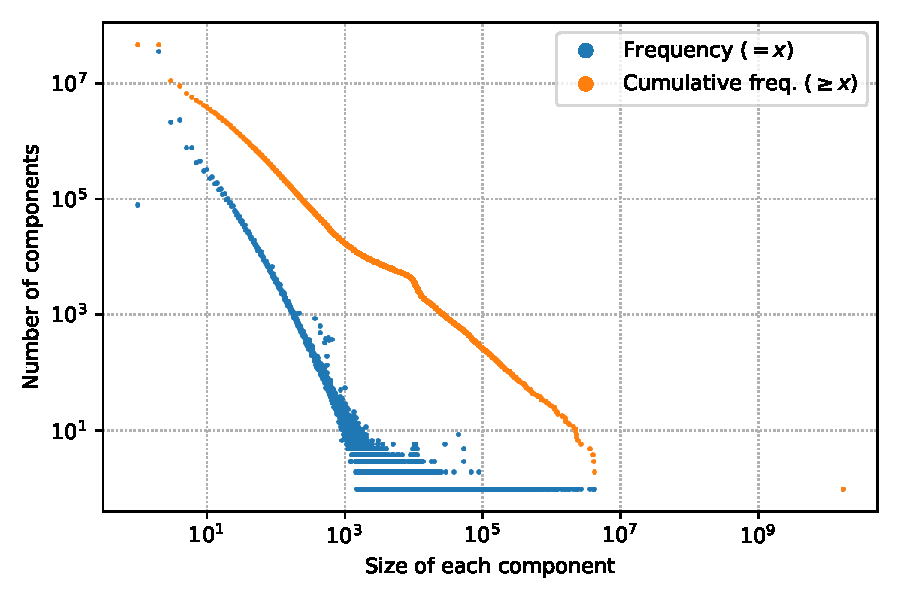
\includegraphics[width=0.9\linewidth]{img/topology/connectedcomponents/dir+cnt}
                \caption{Filesystem layer}
            \end{subfigure}\hfill
            \begin{subfigure}{.49\textwidth}
                \centering
                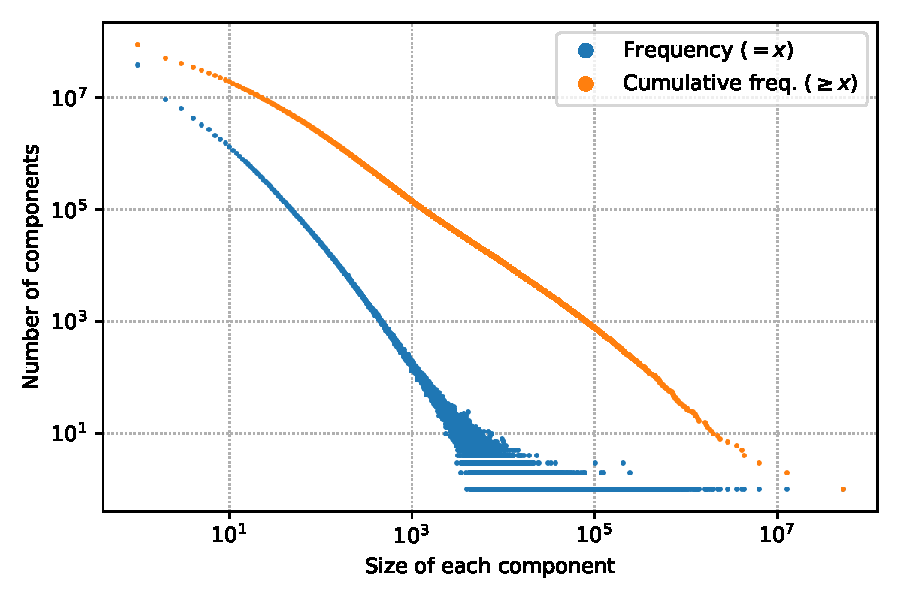
\includegraphics[width=0.9\linewidth]{img/topology/connectedcomponents/rev}
                \caption{Commit layer}
            \end{subfigure}
        \end{figure}

        \begin{tabular}[t]{l r r r}
            \textbf{Layer} & \textbf{\# of WCC}
            & \textbf{Size of largest WCC}
            & \textbf{\% in largest}
            \\
            \hline
            Full graph       & \num{33104255}  & \num{18902683142} & 97.79\% \\
            Filesystem layer & \num{46286502}  & \num{16565521611} & 97.16\% \\
            Commit layer     & \num{88031649}  & \num{51543944}    & 2.61\% \\
        \end{tabular}
    \end{frame}

    \begin{frame}
        \frametitle{Filesystem / commit layer duality}
        \pdfpcnote{%
            To summarize, what's really interesting is the duality between the
            filesystem and the commit layers, they have almost opposite
            topological properties.
            \\\\
            The filesystem layer is very dense and cannot be partitioned easily
            because it has a giant connected component. The files have a
            characteristic depth of less than 10-20 levels, but there's no
            characteristic number of entries in the directories.
            \\\\
            The commit layer is the opposite in almost every way. It's a lot
            sparser, its largest component is rather small which makes it
            possible to partition it. The commit chains are arbitrarily long,
            but commits have a characteristic outdegree of about one, which
            makes them look like long degenerate chains.
        }

        \begin{block}{}
            The filesystem and commit layers have almost opposite topological
            properties.
        \end{block}

        \begin{columns}
            \column{0.5\columnwidth}
            \begin{block}{Filesystem layer}
                \begin{itemize}
                    \item Dense, non-partitionable (giant WCC)
                    \item Characteristic depth
                    \item Arbitrary out-degree
                \end{itemize}
                \begin{center}
                    \scalebox{0.7}{\begin{tikzpicture}
	\begin{pgfonlayer}{nodelayer}
		\node [style=none] (9) at (-3.5, 1.5) {};
		\node [style=none] (10) at (1.5, 1.5) {};
		\node [style=none] (11) at (1.5, 2) {};
		\node [style=none] (12) at (1.5, 5) {};
		\node [style=directory] (13) at (0, 5) {};
		\node [style=directory] (14) at (-1, 4) {};
		\node [style=directory] (15) at (0.5, 4) {};
		\node [style=content] (16) at (-2.25, 3) {};
		\node [style=content] (17) at (-1.5, 3) {};
		\node [style=content] (18) at (-0.75, 3) {};
		\node [style=directory] (19) at (0.5, 3) {};
		\node [style=content] (20) at (0, 2) {};
		\node [style=content] (22) at (-3, 3) {};
		\node [style=content] (23) at (1, 2) {};
	\end{pgfonlayer}
	\begin{pgfonlayer}{edgelayer}
		\draw [style=dashed arrow] (12.center) to (11.center);
		\draw [style=arrow] (13) to (14);
		\draw [style=arrow] (13) to (15);
		\draw [style=arrow] (15) to (19);
		\draw [style=arrow] (14) to (18);
		\draw [style=arrow] (14) to (17);
		\draw [style=arrow] (19) to (20);
		\draw [style=arrow] (19) to (23);
		\draw [style=arrow] (14) to (16);
		\draw [style=arrow] (14) to (22);
		\draw [style=dashed arrow] (12.center) to node [right, align=left] {Characteristic\\depth} (11.center);
		\draw [decorate, decoration={brace,amplitude=10pt}] (10.center) to node [align=center, below=10pt] {Arbitrary\\outdegree} (9.center);
	\end{pgfonlayer}
\end{tikzpicture}
}
                \end{center}
            \end{block}

            \column{0.5\columnwidth}
            \begin{block}{Commit layer}
                \begin{itemize}
                    \item Sparse, partitionable (max WCC = 3\%)
                    \item Arbitrary depth
                    \item Characteristic out-degree (degenerate)
                \end{itemize}
                \begin{center}
                    \scalebox{0.5}{\begin{tikzpicture}
	\begin{pgfonlayer}{nodelayer}
		\node [style=revision] (0) at (0, 0) {};
		\node [style=revision] (1) at (0, 1) {};
		\node [style=revision] (2) at (0, 2) {};
		\node [style=revision] (3) at (0, 3) {};
		\node [style=revision] (4) at (1, 2.5) {};
		\node [style=revision] (5) at (1, 1.5) {};
		\node [style=revision] (6) at (0, 4) {};
		\node [style=revision] (7) at (0, 5) {};
		\node [style=revision] (8) at (1, 3.5) {};
		\node [style=none] (9) at (-0.5, -0.5) {};
		\node [style=none] (10) at (1.5, -0.5) {};
		\node [style=none] (11) at (1.5, 0) {};
		\node [style=none] (12) at (1.5, 5) {};
	\end{pgfonlayer}
	\begin{pgfonlayer}{edgelayer}
		\draw [style=arrow] (1) to (0);
		\draw [style=arrow] (5) to (1);
		\draw [style=arrow] (2) to (1);
		\draw [style=arrow] (4) to (5);
		\draw [style=arrow] (3) to (2);
		\draw [style=arrow] (6) to (3);
		\draw [style=arrow] (3) to (4);
		\draw [style=arrow] (7) to (6);
		\draw [style=arrow] (8) to (4);
		\draw [style=dashed arrow] (12.center) to (11.center);
		\draw [style=dashed arrow] (12.center) to node [right, align=left] {Arbitrary\\depth} (11.center);
        \draw [decorate, decoration={brace,amplitude=10pt}] (10.east) to node [align=center, below=10pt] {Characteristic\\outdegree} (9.west);
	\end{pgfonlayer}
\end{tikzpicture}
}
                \end{center}
            \end{block}
        \end{columns}
    \end{frame}

    \begin{frame}
        \frametitle{Implications for software mining research}
        \pdfpcnote{%
            This has a few implications for software mining research.
            The first one is that there's a wild disparity between the
            different layers that constitute the graph, so they need to be
            studied separately, otherwise the behavior you will observe will be
            dominated by the filesystem layer and you will miss the subtlety of
            the topology of the different layers.
            \\\\
            The second thing to note is that a lot of distributions seem to
            have a high propensity to produce outliers, so we should be careful
            to systematically justify how we filter outliers in empirical
            studies. It also shows that exhaustive studies can be very useful
            to check that results generalize properly.
            \\\\
            Finally, my experiments show that there is no natural way to
            partition the graph in small isolated clusters, which would be
            useful to distribute computations.
        }

        \begin{block}{Layers}
            \begin{itemize}
                \item Large disparity in the topological structure of layers
                \item Important to study layers separately to understand
                    the graph structure
            \end{itemize}
        \end{block}

        \begin{block}{Methodology}
            \begin{itemize}
                % \item High kurtosis / propensity to produce outliers
                \item No obvious threshold to ``filter'' outliers in many
                    distributions
                \item Highlights the importance of exhaustive approaches
            \end{itemize}
        \end{block}

        \begin{block}{Distributed analysis}
            \begin{itemize}
                \item No natural partitioning in small connected components
                \item Need for more subtle approaches?
            \end{itemize}
        \end{block}
    \end{frame}

    \section{Identification of Software Forks}

    \begin{frame}
        \frametitle{Studying software forks}
        \pdfpcnote{%
            The topology analysis is a generic way to analyze any complex
            network, it's domain agnostic. It's very useful to understand the
            fundamental structure of the graph. But we also know that because
            this particular graph shows relationships between deduplicated
            software artifacts, it is semantically structured by code reuse
            patterns, people copying code from one version or one project to
            another. And one way to try to understand this domain-specific
            structure is to study software forks, which are projects built on
            top of existing projects, starting from their codebase but
            continuing the development in parallel.
            \\\\
            In general, studying software forks has many useful applications in
            empirical software engineering, because it helps us understands how
            communities grow and evolve and how that leads to more or less
            successful or healthy projects.
        }

        \begin{block}{}

            \begin{itemize}
                \item Topology analysis of the graph of software development
                    gives us a domain-agnostic understanding of relationships between
                    \emph{deduplicated software artifacts}
                \item This particular graph is structured by
                    \textbf{code reuse patterns}
                \item One way to understand these is to study \textbf{software
                    forks}: projects derived from existing software and being
                    developed independently.
            \end{itemize}

            \footnotesize
            \begin{thebibliography}{swhforks}
                \bibitem{swhforks} Antoine Pietri, Guillaume Rousseau, Stefano Zacchiroli\newblock
                Forking Without Clicking: on How to Identify Software Repository Forks\newblock
                Mining Software Repositories 2020\newblock
            \end{thebibliography}
        \end{block}

        \begin{block}{Applications in software evolution \& software health}
            \begin{itemize}
                \item Finding active and maintained projects
                \item Understanding ``hard'' and ``development'' forks
                \item Identifying criteria for successful forks
            \end{itemize}
        \end{block}
    \end{frame}

                % \item The compressed graph allows us to run exhaustive
                %     quantitative studies on software forks
                % \item Understanding forks is a key research direction in
                %     software health and software evolution

    \begin{frame}
        \frametitle{Previous approaches for studying forks}
        \pdfpcnote{%
            Most studies studying software forks have only looked at platform
            metadata, like what happens when you press the "fork" button on
            collaborative development platforms like GitHub. You can extract
            and study a graph of these relationships from GitHub, but this
            approach is restricted to a single platform. You can't see the code
            reuse patterns that happen between different platforms or even
            different version control systems.\\
            Using the compressed graph, we can try to have a more exhaustive
            approach to identify these forks.
        }

        \begin{block}{}
            \begin{itemize}
                \item Most studies have relied on metadata from collaborative
                    development platforms to identify forks: relationships
                    created by pressing the ``fork'' button
                    \begin{center}
                        
\includegraphics[width=2cm]{img/forkbutton}
                    \end{center}
                \item GitHub provides a graph of forks to parent repositories
                    \begin{center}
                        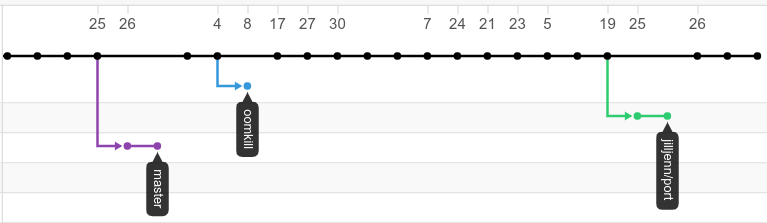
\includegraphics[width=7cm]{img/forknetwork}
                    \end{center}
            \end{itemize}
        \end{block}

        \begin{block}{}
            \begin{itemize}
                \item Restricted to a single platform, relies on external metadata
                \item We can use the \textbf{compressed graph} for a more
                    exhaustive approach
            \end{itemize}
        \end{block}
    \end{frame}

    \begin{frame}
        \frametitle{Intrinsic forks}
        \pdfpcnote{%
            The general idea is that instead of relying on platform metadata,
            we can instead try to find projects that share some development
            history, that we call intrinsic forks. If two different
            repositories have at least one commit in common, we can consider
            that they are forks of each other, without relying on external
            information.
            \\\\
            So we're trying to quantitatively evaluate whether this definition
            is good, how does it compare to the previous approach of using
            platform metadata?
            \\\\
            So I designed an experiment to do this comparison in an exhaustive
            way. I use the compressed graph to identify all the intrinsic forks
            in the graph of software development, then I compare them to the
            ones you get by using the metadata on GitHub.
        }
        \begin{block}{}
            Intuition: \textbf{Intrinsic forks} are software projects
            with \textbf{shared development history}.
        \end{block}

        \begin{block}{}
            \begin{itemize}
                \item Identified by intrinsic DVCS information (= at least one
                    shared commit)
                \item Includes projects for which no forking metadata is present
            \end{itemize}
        \end{block}

        \begin{block}{Research question}
            How do forks from collaborative development platforms compare to
            forks defined by shared development history?
        \end{block}

        \begin{block}{Experimental design}
            We \textbf{identify} intrinsic forks in the graph of development
            history, then quantitatively \textbf{compare} them to forks
            identified by GitHub metadata.
        \end{block}
    \end{frame}

    % \begin{frame}{Methodology}
    %     \pdfpcnote{%
    %     }

    %     \begin{block}{New concepts}
    %         \begin{itemize}
    %             \item \textbf{Fork networks}: repositories connected by
    %                 forking relationships
    %             \item \textbf{Fork cliques}: repositories that are all forks of
    %                 each other
    %         \end{itemize}
    %     \end{block}
    % \end{frame}

    \begin{frame}
        \frametitle{Distribution comparison}
        \pdfpcnote{%
            There are a few considerations on how to cluster similar forks
            together that I detail in the thesis, but basically these are the
            results we get. We see that by using platform specific metadata, we
            miss around 8\% of all the forks. And that's only on two comparable
            datasets, so it doesn't even include the cross-platform forks that
            we could discover using this technique.
            \\\\
            The difference between the two distributions stay mostly positive,
            which indicates that this method is more exhaustive in general. But
            the similarities between the two distributions are also visually
            striking, which indicates that our new definition really matches
            well with the intuitive notion that people have of what a fork
            corresponds to.
            \\\\
            So all in all we show that this technique to identify forks is more
            robust, and can discover forks across different platforms or even
            different VCS.
        }
        \begin{center}
            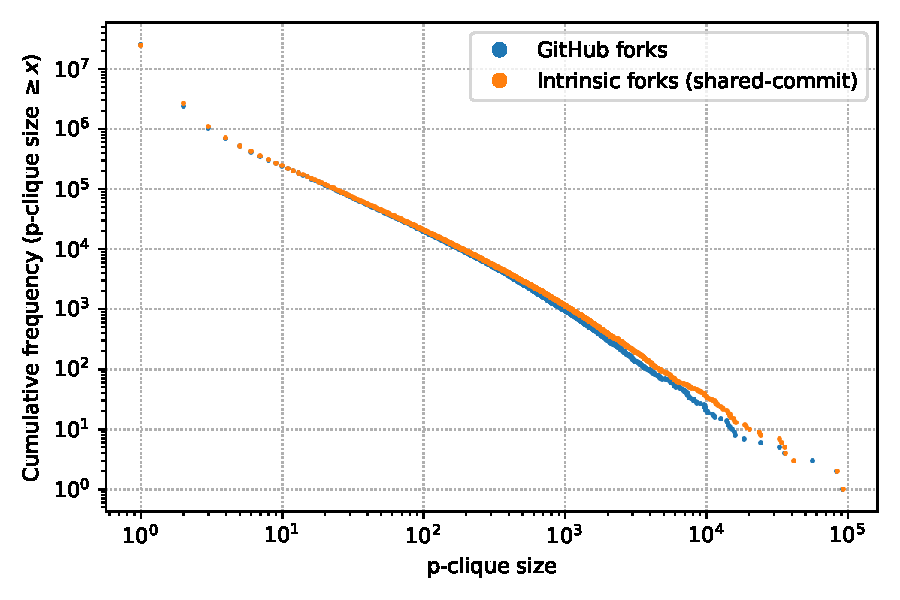
\includegraphics[width=0.5\linewidth]{img/forks/fork-clique-partition-freq-distribution.pdf}
        \end{center}
        \begin{block}{}
            \begin{itemize}
                \item \textbf{8\% of forks missed} when using platform-level
                    metadata
                \item Positive difference ⇒ more exhaustive identification of
                    forks
                \item Distribution similarity ⇒ Matches
                    expectations of what a fork is
                \item Robust approach across platforms and across VCSs
            \end{itemize}
        \end{block}
    \end{frame}

    % \begin{frame}
    %     \frametitle{Implications for software mining research}
    %     \pdfpcnote{%
    %         This study has a few other implications for software mining
    %         research. If we only rely on platform metadata to identify
    %         software forks we will miss a lot of forks, and it might introduce
    %         an important selection bias because we will only ever consider the
    %         forks inside a single platform. The technique we propose to
    %         identify intrinsic forks is more robust, and can uncover forks
    %         across different platforms and even different VCS.
    %     }

    %     \begin{block}{}
    %         \begin{itemize}
    %             \item Relying on forge metadata ⇒ selection bias,
    %                 non-exhaustive
    %             \item Using shared development history uncovers more forks
    %         \end{itemize}
    %     \end{block}

    % \end{frame}

    \section{Conclusion}

    \begin{frame}
        \frametitle{Academic contributions}
        \pdfpcnote{%
            I'll go over a quick summary of my main academic contributions. The
            first thing I've done is to frame the problem by doing a literature
            review of researcher needs, and establishing a roadmap towards
            universal software mining
            \\\\
            I proposed ways to make software development data accessible to
            researchers at three different scales: limited sets of data with
            the Vault and the SwhFS, scale-out processing with the graph
            dataset on various clouds, and a compression approach to analyze
            the graph exhaustively on a single machine.
            \\\\
            Using these platforms, I realized two empirical studies to try to
            understand the structure of the graph, both in a domain-agnostic
            way by computing metrics that characterize its topological
            properties, but also in a domain-specific way, to see how the graph
            is structured by code reuse patterns and software forks.
        }

        \begin{block}{Contextualization}
            \begin{itemize}
                \item Literature review: identify research needs
                \item Roadmap to universal software mining (BENEVOL 2018)
            \end{itemize}
        \end{block}

        \begin{block}{Making software artifacts data available}
            \begin{itemize}
                \item Small scale: Vault, SwhFS (ICSE 2021)
                \item Scale-out: Graph dataset (MSR 2019)
                \item Scale-up: Graph compression (SANER 2020)
            \end{itemize}
        \end{block}

        \begin{block}{Empirical studies on the graph structure}
            \begin{itemize}
                \item Domain-agnostic: topological properties (MSR 2020)
                \item Domain-specific: structure of forks (MSR 2020)
            \end{itemize}
        \end{block}
    \end{frame}

    % \begin{frame}
    %     \frametitle{Empirical findings \& impact on software mining}
    %     \begin{block}{Topology}
    %         \begin{itemize}
    %             \item Disparity between graph layers
    %             \item Graph cannot be partitioned naturally
    %             \item No sound way to filter outliers
    %         \end{itemize}
    %     \end{block}
    %     \begin{block}{Forks}
    %         \begin{itemize}
    %             \item Forks can be identified more exhaustively with shared
    %                 development history
    %             \item They qualitatively fit established notions of what constitutes a ``fork''
    %         \end{itemize}
    %     \end{block}
    % \end{frame}

    \begin{frame}
        \frametitle{Future work}
        \pdfpcnote{%
            The work I presented opens various perspectives for future
            research. The most immediate follow-up would be to make this more
            production-ready so that it can be reused easily.
            \\\\
            Right now the compressed graph works on a static export of the
            dataset, which means there is always a lag with the live data. We
            could try to make this compression incremental to reduce this lag.
            We could also integrate more expressive query languages like GQL or
            Gremlin to make it possible to run more complex queries without
            having to use low-level algorithms.
            \\\\
            Another interesting direction is making improvements to scale-out
            processing. The general idea here is to try to find hybrid
            approaches between the compressed graph and distributed computing.
            For instance we could try to shard the graph efficiently using
            modular decomposition or locality preserving orders like the BFS or
            LLP. It should also be possible to do more integration between the
            two, so that you can transparently perform parts of a computation
            on the compressed graph, and offload the rest on the scale-out
            platforms to maximize efficiency.
            \\\\
            Finally this platform could be used to generate derived graphs that
            are also interesting to software mining researchers, like community
            graphs, commit diffs or dependency graphs. We could compress them
            and make them accessible in the same way.
        }

        \begin{block}{Compressed graph improvements}
            \begin{itemize}
                \item Incremental graph compression
                \item Expressive remote graph querying
            \end{itemize}
        \end{block}
        \begin{block}{Scale-out processing}
            \begin{itemize}
                \item Sharding the graph with modular decomposition,
                    locality-preserving orders…
                \item Integrating the compressed graph with scale-out
                    processing
            \end{itemize}
        \end{block}
        \begin{block}{Generating derived data}
            \begin{itemize}
                \item Community graphs
                \item Commit diffs
                \item Dependency graphs
            \end{itemize}
        \end{block}
    \end{frame}

    \begin{frame}
        \frametitle{Thanks!}

        \begin{block}{}
            \emph{All} this work is open \{source, data, access, …\}.

            \url{https://forge.softwareheritage.org}
            \hfill
            \url{https://github.com/seirl/thesis}
        \end{block}

        \begin{block}{}
            \tiny
            \begin{itemize}
                \item \fullcite{swh-benevol2018-universal-analysis}
                \item \fullcite{swh-msr2019-dataset}
                \item \fullcite{msr-2020-challenge}
                \item \fullcite{saner-2020-swh-graph}
                \item \fullcite{swh-msr2020-forking}
                \item \fullcite{msr-2020-topology}
                \item \fullcite{swh-2021-swhfs}
            \end{itemize}
        \end{block}
    \end{frame}
\end{document}
